%Copyright 2014 Jean-Philippe Eisenbarth
%This program is free software: you can 
%redistribute it and/or modify it under the terms of the GNU General Public 
%License as published by the Free Software Foundation, either version 3 of the 
%License, or (at your option) any later version.
%This program is distributed in the hope that it will be useful,but WITHOUT ANY 
%WARRANTY; without even the implied warranty of MERCHANTABILITY or FITNESS FOR A 
%PARTICULAR PURPOSE. See the GNU General Public License for more details.
%You should have received a copy of the GNU General Public License along with 
%this program.  If not, see <http://www.gnu.org/licenses/>.

%Based on the code of Yiannis Lazarides
%http://tex.stackexchange.com/questions/42602/software-requirements-specification-with-latex
%http://tex.stackexchange.com/users/963/yiannis-lazarides
%Also based on the template of Karl E. Wiegers
%http://www.se.rit.edu/~emad/teaching/slides/srs_template_sep14.pdf
%http://karlwiegers.com
\documentclass{scrreprt}

\usepackage{listings}
\usepackage{color}
\usepackage{underscore}
\usepackage[bookmarks=true]{hyperref}
\usepackage[utf8]{inputenc}
\usepackage[english]{babel}
\usepackage{booktabs}
\usepackage[table,xcdraw]{xcolor}
\usepackage{graphicx}
\usepackage{placeins}
\usepackage{ltxtable} 
\usepackage{listings}% http://ctan.org/pkg/listings
\usepackage{amsmath}

\usepackage{algorithm}
\usepackage{algorithmicx}
\usepackage{algcompatible}

\usepackage[noend]{algpseudocode}
\usepackage{fixltx2e}
\usepackage{hyperref}

\definecolor{codegreen}{rgb}{0,0.6,0}
\definecolor{codegray}{rgb}{0.5,0.5,0.5}
\definecolor{codepurple}{rgb}{0.58,0,0.82}
\definecolor{backcolour}{rgb}{0.95,0.95,0.92}
 
\lstdefinestyle{mystyle}{
    backgroundcolor=\color{backcolour},   
    commentstyle=\color{codegreen},
    keywordstyle=\color{magenta},
    numberstyle=\tiny\color{codegray},
    stringstyle=\color{codepurple},
    basicstyle=\footnotesize,
    breakatwhitespace=false,         
    breaklines=true,                 
    captionpos=b,                    
    keepspaces=true,                 
    numbers=left,                    
    numbersep=5pt,                  
    showspaces=false,                
    showstringspaces=false,
    showtabs=false,                  
    tabsize=2
}
 
\lstset{style=mystyle}

\graphicspath{ {images/} }
\hypersetup{
    bookmarks=false,    % show bookmarks bar?
    pdftitle={Software Requirement Specification},    % title
    pdfauthor={Jean-Philippe Eisenbarth},                     % author
    pdfsubject={TeX and LaTeX},                        % subject of the document
    pdfkeywords={TeX, LaTeX, graphics, images}, % list of keywords
    colorlinks=true,       % false: boxed links; true: colored links
    linkcolor=blue,       % color of internal links
    citecolor=black,       % color of links to bibliography
    filecolor=black,        % color of file links
    urlcolor=purple,        % color of external links
    linktoc=page            % only page is linked
}%
\def\myversion{1.0 }
\date{}
%\title
\usepackage{hyperref}

\makeatletter
\def\BState{\State\hskip-\ALG@thistlm}
\makeatother
\begin{document}

\begin{flushright}
    \rule{16cm}{5pt}\vskip1cm
    \begin{bfseries}
        \Huge{Small Scale Parellel Programming\\ Assignment}\\
       
        \vspace{1.9cm}
        \LARGE{Version \myversion approved}\\
        \vspace{1.9cm}
        Prepared by Wiktor Bednarek\\
        \vspace{1.9cm}
        Supervisor Dr Salvatore Filippone \\
        \vspace{1.9cm}
        Cranfield University\\
        \vspace{1.9cm}
        \today\\
    \end{bfseries}
\end{flushright}

\tableofcontents


\chapter*{Revision History}

\begin{center}
    \begin{tabular}{|c|c|c|c|}
        \hline
	    Name & Date & Reason For Changes & Version\\
        \hline
	    Wiktor Bedanrek & 06.09.2017 & First version & 1\\
        \hline
	    Wiktor Bedanrek & 13.07.2017 & New version adjustments - tests & 1.1\\
        \hline
         Wiktor Bedanrek & 14.07.2017 & Code improvement& 1.2\\
        \hline
         Wiktor Bedanrek & 15.07.2017 & Summary design specification& 1.3\\
        \hline
         Wiktor Bedanrek & 16.07.2017 & New version adjustments - update& 1.4\\
        \hline
          Wiktor Bedanrek & 17.07.2017 & Use cases and code diagrams& 1.55\\
        \hline
          Wiktor Bedanrek & 18.07.2017 & Performance and unit tests chapter& 1.7\\
        \hline
    \end{tabular}
\end{center}

\chapter{Introduction}
Modern computation demands still more and more resources. Users, industry or companies process enormous amount of data every day. When it comes to computation thanks to technological development we can solve complex problems efficiently and fast. But since last decade programmers have to get acquired with a new type of problems solving which is parallelism. That concept is widely used these days especially in GPUs. We will show huge benefits of solving mathematical problems in parallel. 
\section{Purpose}
Purpose of this paper is to show solution and results of martix by "tall" dense matrix multiplication. It will be implemented using parallel programming interfaces Open Multi-Processing (OpenMP) and Nvidia CUDA.  

Kernel will be capable to compute
\begin{equation} \label{eu_eqn}
X \leftarrow AX
\end{equation}

A is a sprase matrix. We will store matrix in a following formats:
\begin{enumerate}
\item CSR - Compressed Sparse Row
\item ELL - ELLPACK

\end{enumerate}




\section{Document Conventions}
All requirements information are given in this paper. Chapters are divided into sections containing tables and results as a images.

The most crucial is to provide reader following informations:
\begin{itemize}
	\item Solution description
	\item Comparison between solutions
	\item Results of the tests
	\item Performance results
\end{itemize}  


The next important convection is features priority. The following table will explain priority scale and importance .

\begin{table}[h!]
\centering
\caption{Priority table}
\label{my-label}
\begin{tabular}{|l|l|}
\hline
\textbf{Priority}                                                & \textbf{Description}                                                                                                                                                                                                                                                                                                            \\ \hline
\begin{tabular}[c]{@{}l@{}} 1 \end{tabular} & \begin{tabular}[c]{@{}l@{}} Very low priority software feature. \\ It has no affect for the proper program run.  The program is going to work  \\ without this feature implementation. Example: minor code comments.  \end{tabular}                                                                                                        \\ \hline
2                                                        & \begin{tabular}[c]{@{}l@{}} Low priority software feature.  \\ The software is going to work properly without its implementation. \\ Example: vectors or arrays displaying fuctions created to check results. \\ They will be deleted in the final code or replaced by the tests.\end{tabular}                                                                                                                                                                   \\ \hline
3                                                    & \begin{tabular}[c]{@{}l@{}} Low priority software feature. \\ The feature has insignificant affect to overall software. This feature has no \\ impact on results but it could help in maintaining the code like: refactorization\\ \end{tabular}                                                                                                                     \\ \hline
4                                                  & \begin{tabular}[c]{@{}l@{}} Lower-Medium priority software feature.\\ The feature might give some improvement like better results displaying or saving \\ them to the file.\end{tabular} \\ \hline
5                                                        & \begin{tabular}[c]{@{}l@{}} Medium priority software feature.\\ That functionality should be implemented; without it, software might have minor \\ issues like slightly lower program performance. The program is \\  going to  run  properly without its implementation.\end{tabular}                                                                                                                                                                   \\ \hline
6                                                        & \begin{tabular}[c]{@{}l@{}} Upper-Medium priority software feature.  \\ This implementation is important in order to have consisted software.   \end{tabular}                                                                                                                                                                   \\ \hline
7                                                        & \begin{tabular}[c]{@{}l@{}} High priority software feature.  \\ This functionality significantly helps to maintain software and it contains \\ features like performance tests.  \end{tabular}                                                                                                                                                                   \\ \hline
8                                                        & \begin{tabular}[c]{@{}l@{}} Very High priority software feature.   \\ The Feature has to be implemented. It significantly affects for program results.\end{tabular}                                                                                                                                                                   \\ \hline
9                                                        & \begin{tabular}[c]{@{}l@{}} Very High priority software feature.  \\ Without this feature the program mostly probably is going to have serious issues \\ like poor  performance or invalid results.\end{tabular}                                                                                                                                                                   \\ \hline
10                                                        & \begin{tabular}[c]{@{}l@{}} The highest priority software feature.   \\ The most crucial program features - core functions. \\ The program is not going to run without them. Example: CUDA and  OpenMP \\ computation of  martix by "tall" dense matrix multiplication.\end{tabular}                                                                                                                                                                   \\ \hline
\end{tabular}
\end{table}
\FloatBarrier


    

\section{Intended Audience and Reading Suggestions}

Document has detailed information about solution and it is designed to be clear to understand . For high coefficient of transparency all important data are presented tables.
This software is intended to use by research staff in scientific facilitates or students which would like to deepen their parallel programming knowledge.
\\

\begin{table}[h!]
\centering
\caption{Informations for the specified audience in the following paper}
\label{my-label}
\begin{tabular}{|l|l|}
\hline
\textbf{Student}                                                & \textbf{Informations to find}                                                                                                                                                                                                                                                                                                            \\ \hline
\begin{tabular}[c]{@{}l@{}}Researcher\end{tabular} & \begin{tabular}[c]{@{}l@{}} Results of sparse matrix-vector product kernel  \\ Idea how powerful presented solution is and how to use it \\ in a different potential problem \end{tabular}                                                                                                        \\ \hline
Student                                                        & \begin{tabular}[c]{@{}l@{}} Student can find information of algorithm implementation  \\ This knowledge might be helpful for his potential parallel programming \\ approach purposes.\end{tabular}                                                                                                                                                                   \\ \hline
Industry                                                     & \begin{tabular}[c]{@{}l@{}}Similar like in a students case  Additionally information \\ about special features available only for Researchers like: \\ accelerated nodes for GPU computation.\end{tabular}                                                                                                                     \\ \hline
Other IT                                                    & \begin{tabular}[c]{@{}l@{}}Details about Special IT support functions e.g. Efficient algorithms   \\ usage  in computer graphics, image processing or other \\  multi thread computations\end{tabular} \\ \hline
\end{tabular}
\end{table}
\FloatBarrier

\section{Used hardware}
All tests were performed at following configuration:

\begin{table}[h!]
\centering
\caption{Computer hardware used in the project}
\label{my-label}
\begin{tabular}{|l|l|}
\hline
\textbf{Type of hardware}      & \textbf{Description} \\ \hline                                                                                                                                                                                  
Processor        & \begin{tabular}[c]{@{}l@{}}AMD Phenom II X4 955 QuadCore 3.2GHz\end{tabular} \\ \hline                                                                                                   
RAM              & \begin{tabular}[c]{@{}l@{}}4096 MB DDR3\end{tabular} \\ \hline
GPU     & \begin{tabular}[c]{@{}l@{}}Nvida GeForce GT 730 1GB\end{tabular} \\ \hline
Hard drive     & \begin{tabular}[c]{@{}l@{}}SSD 256 GB\end{tabular} \\ \hline
\end{tabular}
\end{table}
\FloatBarrier


\section{Operating Environment}



System was developed for following working environment:
\\
\\
Software:
\begin{itemize}
\item  Windows 7
\item  Visual Studio 2015 with Nsight extension

\end{itemize}
 





\section{Project Scope}

This project provides computation of matrix by "tall" dense matrix multiplication. All computations are done in parallel using two technologies OpenMP and Nvida CUDA. In this paper we are going to use matrices from external internet resource available at the website //www.cise.ufl.edu/research/sparse especially at \\ \textbf{https://www.cise.ufl.edu/research/sparse/matrices/list_by_name.html}. \\ Because up to date 14.07.2017 not all of matrices are available at the last website, the most of the matrices were collected from \\ \textbf{http://yifanhu.net/GALLERY/GRAPHS/search.html}. \\ 
Matrices are downloaded in Matrix Market format (MM) and in the program transformed into CSR o ELLPack format. Having that stored matrices we perform  matrix by "tall" dense matrix multiplication using OpenMP or Cuda technology. Performance is checked by a proper tests.

\begin{table}[h!]
\centering
\caption{Basic scope of project}
\label{my-label}
\begin{tabular}{|l|l|}
\hline
\textbf{Name}      & \textbf{Description}                                                                                                                                                                                  \\ \hline
Researcher        & \begin{tabular}[c]{@{}l@{}}Displaying results for selected matrix\\ Calculates sparse matrix-vector product \\ and shows its performance \end{tabular}                                                                                                   \\ \hline
Student             & \begin{tabular}[c]{@{}l@{}}  View performance results for different\\  problems both in OpenMP and CUDA\\ \end{tabular} \\ \hline

\end{tabular}
\end{table}
\FloatBarrier


\section{References}

\begin{itemize}
\item http://docs.nvidia.com/cuda/cuda-c-best-practices-guide/index.html. Retrieved June 2017.
\item https://developer.download.nvidia.com/CUDA/training/NVIDIA_GPU_Computing_Webinars_Further_CUDA_Optimization.pdf. Retrieved May 2017.
\item http://www.openmp.org/resources/tutorials-articles/. Retrieved June 2017.
\item http://www.hpctoday.com/hpc-labs/explicit-vector-programming-with-openmp-4-0-simd-extensions/. Retrieved June 2017.
\end{itemize}


\chapter{Summary design specification}

\section{Purpose of the project}
The main feature of our solution is implement the kernel that is capable of computing martix by "tall" dense matrix multiplication. We are using two main parallel technlgies in our solution Open Multi-Processing (OpenMP) and Nvidia CUDA.  

Kernel will be capable to compute:
\begin{equation} \label{eu_eqn}
X \leftarrow AX
\end{equation}
\\
Where:
\\
A is a sprase matrix stored in the following formats:
\begin{enumerate}

\item CSR - Compressed Sparse Row
\item ELL - ELLPACK
\end{enumerate}

X and Y are "tall" dense matrices what stands for matrices with limited number of columns. Having a given size M of the matrix A we consider X and Y of size as follows: \\
M x 2, M x 4, M x 3 and M x 8.
\\
Considering product of sparse matrix A by an M x K, there will be 2 x NZ x k number of floating point operations.

Our solutions will be tested with the relevant tests. We will check influence of the performance evaluated in the Millions of Floating point Operations Per Second (MFLOPS) depended on number of columns. 

\section{Scope}
Creating the testing simulation that is capable of compute matrix by "tall" dense matrix multiplication, perform all relevant tests and provide the results at the output. We are also going to show results in the following paper. 
\\
At the beginning simulation software will be capable of read and transform Matrix Market format into CSR and ELLPack formats. basing on that formats we will consider kernel matrix by "tall" dense matrix multiplication implemented in Nvdia Cuda. Also another parallel implementation going to be performed in OpenMP. Results will be compared with single thread or single running solution.
\\
Appropriate conclusions will be given at the end of the paper.

\section{Stockholders and indented audience}



\section{Solution details}

\subsection{Code map}

Code map helps to understand all connections  within solution scope. It shows what impact and how connected are classes of functionalities in our solution. Most of the functionalities are dependent on others, below diagram will explain how our software is designed.


\begin{figure}[h!]
\label{CodeMap}
\centering
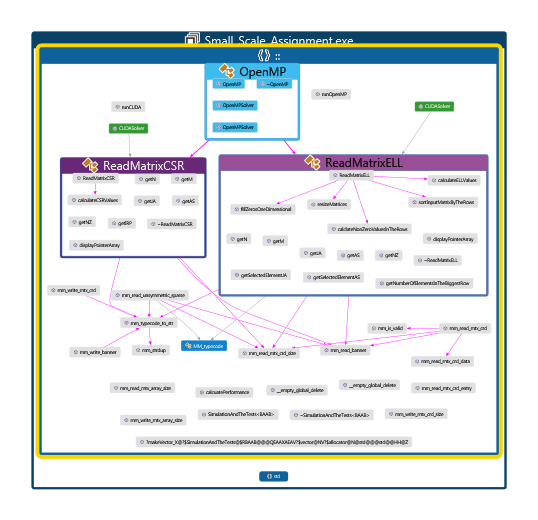
\includegraphics{CodeMap.PNG}
\caption{Code map of our solution}
Source: Own image
\end{figure}
\FloatBarrier


On above figure \ref{CodeMap} we can observe various connections. For instance We have to main classes responsible for transforming Matrix Market (MM) format into CSR and ELLPack. Those classes are: 
\\
\begin{itemize}
\item ReadMatrixCSR - for MM to ELL format transform
\item ReadMatrixELLPack - for MM to CSR format transform
\end{itemize}

They are connected with the functions from external \textit{mmio} library and what is the most important those classes are used further by the main solution functionality i.e. OpenMP (in the light blue frame) parallel class that has implemented functionalities for the matrix by "tall" dense matrix multiplication. That class requires in the first order the ReadMartixCSR or ReadmatrixELL object for demanded computation. 
\\
Those two MM matrix transformation classes are also used by CUDASolver functions, highlighted in green, which are like OpenMP responsible for the matrix by "tall" dense matrix multiplication. Those two overloaded functions require ReadMartixCSR or ReadmatrixELL object for further computation  respectively.

\subsection{Class diagram}

In the project concept the view called class diagram should be created. Below class diagram presents all class in the project and its functions. 

\begin{figure}[h!]
\label{ClassDiagram}
\centering
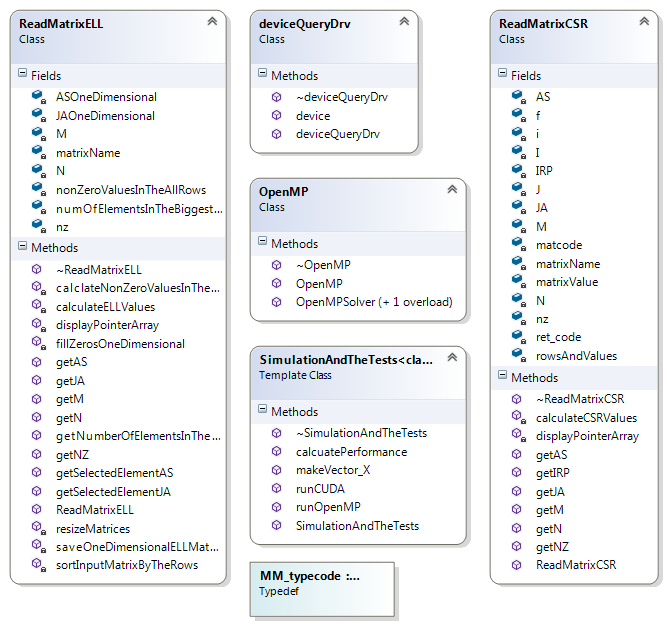
\includegraphics{ClassDiagram.PNG}
\caption{Class diagram of our solution}
Source: Own image
\end{figure}
\FloatBarrier

The solution contains the main classes:
\begin{itemize}
\item ReadMatrixCSR - for MM to ELL format transform
\item ReadMatrixELLPack - for MM to CSR format transform
\item OpenMP class - responsible for OpenMP parallel matrix by "tall" dense matrix multiplication
\item SimilationAndTheTests class - responsible for running creating X matrix and envoking CUDA and OpenMP computations
\item deviceQueryDrv class - external class responsible for reading CUDA device parameters like CUDA Device Total Memory, Tolat amount of global memory, GPU Max Clock rate, Memory Clock rate, Number of CUDA cores, Warp size etc.
\end{itemize}


\textbf{Apart form object oriented code our solution also contains:}

\begin{itemize}
\item main function - determines OpenMP numner of thrads to run and for CUDA size and number of blocks that will be used. Also it read Warp size of used CUDA device. In main fucntion we run whole simulation.

\item mmio - external software from \textit{http://math.nist.gov/MatrixMarket/} for reading matrices from file into memory

\item CUDASolver.cu - set of functions to run CUDA parallel martix by "tall" dense matrix multiplication.

\end{itemize}


\subsection{Use Case diagram}

\begin{figure}[h!]
\label{UseCaseDiagram}
\centering
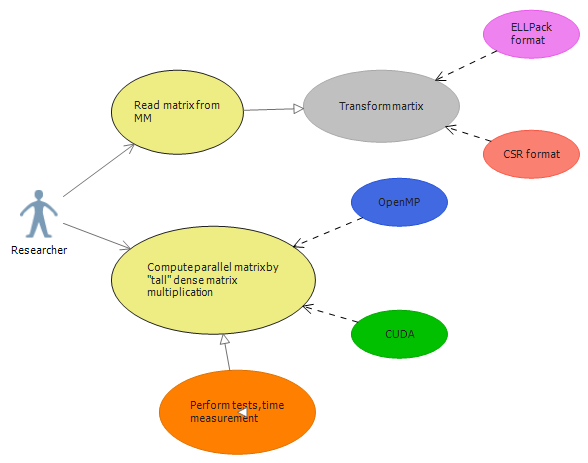
\includegraphics{UseCaseDiagramResearcher.PNG}
\caption{Use Case diagram of our solution}
Source: Own image
\end{figure}
\FloatBarrier

\chapter{Test Matrices}

To perform our simulation test martrices had to be provided. In the following matrix by "tall" dense matrix multiplication problem we used matrices from the websites: \\
\textbf{https://www.cise.ufl.edu/research/sparse/matrices/list_by_name.html} \\
and \\
\textbf{http://yifanhu.net/GALLERY/GRAPHS/search.html}

In this parer we used the following matrices:




\setlength{\arrayrulewidth}{1mm}
\setlength{\tabcolsep}{12pt}
\renewcommand{\arraystretch}{3}
 
\newcolumntype{s}{>{\columncolor[HTML]{AAACED}} p{2cm}}
 
\arrayrulecolor[HTML]{DB5800}

\begin{longtable}[h!]{ |s|p{2cm}|p{1.3cm}|p{1.3cm}|p{1.5cm}|p{2cm}|p{0.5cm}|  }
\caption{Matrices used in the project and the tests} \\
\hline


\rowcolor{lightgray} \multicolumn{7}{|c|}{Matrices List} \\
\hline

Matrix name & Author &Rows &Cols &Nonzeros & Description & Avai-labi-lity \\
\hline
cage4 & A. van Heukelum, T. Davis &9 & 9 &49 & directed weighted graph & \cellcolor[HTML]{28A828} Yes   \\

mhda416 & A. Booten, M. Kooper, H. van der Vorst, S. Poedts, J. Goedbloed &416 & 416 &8,562 & electromagnetics problem & \cellcolor[HTML]{28A828} Yes   \\
mcfe & 	M. Carlsson &765 & 765 &24382 & 2D/3D problem & \cellcolor[HTML]{28A828} Yes   \\
olm1000 & 	K. Meerbergen &1000 & 1000 &3996 & computational fluid dynamics problem & \cellcolor[HTML]{28A828} Yes   \\
adder_dcop_32 & 	R. Hoekstra &1813 & 1813 &11246 & subsequent circuit simulation problem & \cellcolor[HTML]{28A828} Yes   \\
west2021 & A. Westerberg &2021 & 2021 &7310 & chemical process simulation problem & \cellcolor[HTML]{28A828} Yes   \\
rdist2 & 	S. Zitney &3198 & 3,198 &56,834& chemical process simulation problem & \cellcolor[HTML]{28A828} Yes   \\
cant & unknown &62451& 62451 &4,007383 & 2D/3D problem & \cellcolor[HTML]{28A828} Yes   \\
olafu & 	H. Simon &16,146 & 16,146 &1,015,156 & 	structural problem & \cellcolor[HTML]{28A828} Yes   \\
Cube_Coup_dt0 & C. Janna, M. Ferronato &2,164,760 & 2,164,760 &124,406,070 & structural problem &\cellcolor[HTML]{28A828} Yes   \\
ML_Laplace & C. Janna, M. Ferronato, G. Pini &377,002 & 377,002 &27,582,698 & structural problem & \cellcolor[HTML]{28A828} Yes   \\
bcsstk17 & M. Will &10,974 & 10,974 &428,650 & structural problem & \cellcolor[HTML]{28A828} Yes   \\
mac_econ_fwd500 & 	unknown &206,500& 206,500 &1,273,389 & 	economic problem &\cellcolor[HTML]{28A828} Yes   \\
mhd4800a & 	A. Booten, M. Kooper, H. van der Vorst, S. Poedts, J. Goedbloed &4,800 & 4,800 &102,252 & electromagnetics problem & \cellcolor[HTML]{28A828} Yes   \\
cop20k_A & unknown &121,192 & 121,192 &2,624,331& 	2D/3D problem & \cellcolor[HTML]{28A828} Yes   \\
af23560 & 	A. Mahajan &23,560 & 23,560 &460,598 & computational fluid dynamics problem & \cellcolor[HTML]{28A828} Yes   \\
lung2 & S. Norris &109,46 &109,46 &492,564 & omputational fluid dynamics problem & \cellcolor[HTML]{28A828} Yes   \\
PR02R & F. Pacull &161,070& 161,070 &8,185,136 & computational fluid dynamics problem & \cellcolor[HTML]{28A828} Yes   \\
FEM_3D_thermal1 & 	I. Botonakis &17,880 & 17,880 &430,74 & thermal problem& \cellcolor[HTML]{28A828} Yes   \\
thermal1 & D. Schmid &82,654 & 82,654 &574,458 & thermal problem & \cellcolor[HTML]{28A828} Yes   \\
thermal2 & 	D. Schmid &1,228,045 & 1,228,045 &8,580,313& thermal problem & \cellcolor[HTML]{28A828} Yes   \\
thermomech_TK & I. Botonakis &102,158& 102,158 &711,558& thermal problem & \cellcolor[HTML]{28A828} Yes   \\
nlpkkt80 & O. Schenk, A. Waechter, M. Weiser &1,062,400 & 1,062,400 &28,192,672 & optimization problem & \cellcolor[HTML]{28A828} Yes   \\
webbase-1M & 	unknown &1,000,005 & 1,000,005 &3,105,536 & weighted directed graph & \cellcolor[HTML]{28A828} Yes   \\
dc1 & T. Lehner &116,835 & 116,835 &766,396 & circuit simulation problem sequence&\cellcolor[HTML]{28A828} Yes   \\
amazon0302 & 	J. Leskovec, L. Adamic and B. Adamic &262,111 & 262,111 &1,234,877 & directed graph & \cellcolor[HTML]{28A828} Yes   \\
af_1_k101 & AutoForm Eng. &503,625 & 503,625 &17,550,675 & structural problem & \cellcolor[HTML]{28A828} Yes   \\
roadNet-PA & 	J. Leskovec, K. Lang, A. Dasgupta, M. Mahoney &1,090,920 & 1,090,920 &3,083,796 & 	undirected graph & \cellcolor[HTML]{28A828} Yes   \\

\hline
\end{longtable}
\FloatBarrier



All above matrices present various problems like optimization problem, computational fluid dynamics problem, economic problem, structural problem , subsequent circuit simulation problem or chemical process simulation problem etc.
\\
We are downloading those matrices in Matrix Market format. Those files contains matrix with specified its number of rows, columns and number of non zeros values. For instance we have the following lung2.mtx snippet:

\begin{lstlisting}[language=TeX]
%%MatrixMarket matrix coordinate real general
%-------------------------------------------------------------------------------
% UF Sparse Matrix Collection, Tim Davis
% http://www.cise.ufl.edu/research/sparse/matrices/Norris/lung2
% name: Norris/lung2
% [S.Norris, Univ. Auckland. Coupled temp,water vapour transport in lung]
% id: 894
% date: 2003
% author: S. Norris
% ed: T. Davis
% fields: title A name id date author ed kind
% kind: computational fluid dynamics problem
%-------------------------------------------------------------------------------
109460 109460 492564
1 1 9.670098233764655e-8
3 1 -2.936128058287621e-7
1 2 .23174301878262243
2 2 85.78494352552866
3 2 .057935754695655574
4 2 -248.92213269262265
1 3 3.120410728396386e-7
3 3 9.670098233764655e-8
5 3 -2.936128058287621e-7
1 4 .057935754695655574
2 4 260.88752948616593
3 4 .23174301878262243
4 4 85.78494352552866
5 4 .057935754695655574
6 4 -248.92213269262265
3 5 3.120410728396386e-7
5 5 9.670098233764655e-8
7 5 -2.936128058287621e-7
3 6 .057935754695655574
4 6 260.88752948616593
5 6 .23174301878262243
6 6 85.78494352552866
7 6 .057935754695655574
8 6 -248.92213269262265
5 7 3.120410728396386e-7
7 7 9.670098233764655e-8
9 7 -2.936128058287621e-7
5 8 .057935754695655574
6 8 260.88752948616593
7 8 .23174301878262243
8 8 85.78494352552866
9 8 .057935754695655574
10 8 -248.92213269262265
7 9 3.120410728396386e-7
9 9 9.670098233764655e-8
11 9 -2.936128058287621e-7
7 10 .057935754695655574
8 10 260.88752948616593
9 10 .23174301878262243
...
\end{lstlisting}

As we can see at the beginning we have number of rows: 109460; columns: 109460 and non zero values: 492564.
\\
The first line contains: \\
\begin{lstlisting}[language=TeX]
1 1 9.670098233764655e-8
\end{lstlisting}
which stand for as follows two first numbers shows where the first-line value is placed in the matrix i.e. 1 1 means that value 9.670098233764655e-8 is placed at the first row and the first column in that matrix.


\chapter{Storing matrices in Compressed Row Storage (CSR) and ELLPACK formats}
In our software on of the requirement is to store downloaded from the Internet matrices into the CSR and ELLPac formats. In order to do that we need to transform data from the Matrix Market matrices to CSR and ELLPack formats.
In the following section we will explain our approach of performing matrix transformation to the required formats.

\section{Prerequisites}
First of all we need to use external reading matrices software. It should be able to read a matrix from the Matrix Market format file and store it into computer's memory. That kind of tool for C/C++ languages is available at: \\
\textbf{http://math.nist.gov/MatrixMarket/mmio-c.html} 
\\
\\
We need to download two files:
\begin{itemize}
\item  mmio.h
\item  mmio.c

\end{itemize}

Those contains various functions that are necessary to read our MM format matrix. It is also recommended to look at example files available on the same website.


\section{Creating CSR format matrix}

\subsection{Understanding CSR}

Compressed Row Storage (CSR) is one of matrix storage formats. We are going to consider he following matrix: 

\begin{equation} \label{cage4}
a_{M,N} = 
 \begin{pmatrix}
  a_{1,1} & a_{1,2} & \cdots & a_{1,N} \\
  a_{2,1} & a_{2,2} & \cdots & a_{2,N} \\
  \vdots  & \vdots  & \ddots & \vdots  \\
  a_{M,1} & a_{M,2} & \cdots & a_{M,N} 
 \end{pmatrix} 
\end{equation}


 As en example we will consider cage4.mtx matrix. In this situation the CSR M x N matrix with NZ non-zero entries this format has the following parameters:
\\
\\
\textbf{ M} - number of rows
 \\
 \\
\textbf{ N} - number of columns
 \\
 \\
 \textbf{IRP(1:M+1)} - Array/vector of pointers that shows how many more non-zero values are in the selected row than in the previous one. The first element of that array is 0 for C++ or 1 in the Matlab style. \\
In the cage4 matrix example IRP vector has folllowing values:
\\
0 5 10 15 20 26 32 38 44 49 
\\
\\
\textbf{JA(1:NZ)} - Array/vector of indices of columns in which non-zero values are stored. 
\\
How many non-zero values are in the selected column, that many times this column index will be placed the JA array. Considering that a\textsubscript{1,1} matrix element is the value in the left-top matrix corner, we are searching for non-zero values going down with rows a\textsubscript{1,1}...a\textsubscript{M,1}. after finding all NZ values in a selected column, we are searching in that order all NZ values in the columns a\textsubscript{1,1}...a\textsubscript{1,N}. \\


In cage4 matrix example we have:
\\
JA : 0 1 3 4 7 0 1 2 4 5 1 2 3 5 6 0 2 3 6 7 0 1 4 5 6 8 1 2 4 5 7 8 2 3 4 6 7 8 0 3 5 6 7 8 4 5 6 7 8 
\\
\\
\textbf{AS} - Array/vector of the following non-zero values. 
\\
When 1 x 1 matrix element is the one in the left-top matrix corner, the following AS values are the next non-zero matrix values to the right from the (1 x 1) NZ matrix value. Later going down with the rows, analogically all non-zero values from the left to the right from each row are put into AS vector.
\\
Listed AS values in CSR format from cage4.mtx look as follow:
\begin{lstlisting}[language=TeX]
AS has folllowing values: 0.75 0.137458 0.112542 0.137458 0.112542 
0.0750277 0.687569 0.112542 0.0750277 0.112542 0.091639 0.666667 
0.0750277 0.091639 0.0750277 0.091639 0.137458 0.729097 0.137458
0.091639 0.0375138 0.0375138 0.537514 0.137458 0.112542 0.25
0.0458195 0.0458195 0.0750277 0.445875 0.0750277 0.150055 
0.0375138 0.0375138 0.091639 0.470792 0.091639 0.183278 0.0458195 
0.0458195 0.137458 0.112542 0.545819 0.25 0.0833333 0.0750277
0.091639 0.0833333 0.166667 
\end{lstlisting}



\subsection{CSR implementation approach}

In order to implement and transform few steps had to be done. Below pseudo code will explain our apporach.

\begin{algorithm}
\caption{Matrix Market to CSR transformation approach}\label{euclid}
\begin{algorithmic}[1]
\Procedure{MM to CSR}{}
\State Read MM matrix using "mmio" external software
\State Load to memory M Rows form "mmio" external software
\State Load to memory N Columns form "mmio" external software
\State Load to memory NZ non-zero number of values form "mmio" external software
 \For{\texttt{i = 0; i < NZ; ++i}}
        \State Load to memory NZ[i] non-zero values form "mmio" external software
		\State Load to memory I[i] matrix values positions form "mmio" external software
		\State Load to memory J[i] matrix values positions  form "mmio" external software
      \EndFor

\\
\State //Resize JA, IRP and AS pointer arrrys
\State $JAsize \gets NZ$.
\State $IRPsize \gets M+1$.
\State $ASsize \gets NZ$.
\State //Create C++ std::tuple type value
 \For{\texttt{i = 0; i < NZ; ++i}}
        \State $tuple[i] \gets maketuple(I[i], J[i], NZ[i])$
      \EndFor
\State
\State Sort tuple values by the rows
\State
\State $IRPValue \gets 0$.
\State $IRPPos \gets 0$.
\State $columnNumber \gets J[0]$.
 \For{\texttt{i = 0; i < NZ; ++i}}
		\State //Create AS vector
        \State $AS[i] \gets getMatrixValueFromTuple(NZ[i])$
        \State //Create JA vector
         \State $JA[i] \gets getColumnFromTuple(J[i]))$
         \State //Create IRP vector
         \If {$getRowFromTuple(I[i])) = IRPPos$}
		\State $IRPValue \gets IRPValue+1$.
		 \Else
		 \State $IRPPos \gets IRPPos+1$.
		 \State $IRP[IRPPos] \gets IRPValue$.
		\While {$getRowFromTuple(I[i])) != IRPPos$}
		\State $IRPPos \gets IRPPos+1$.
		 \State $IRP[IRPPos] \gets IRPValue$.
		 \EndWhile
		 \State $IRPValue \gets IRPValue+1$.

		\EndIf
      
      \EndFor

\EndProcedure
\end{algorithmic}
\end{algorithm}
\FloatBarrier


\section{Creating ELLPack format matrix}

ELLPack is fomat which describes M x N matrix with NZ entries.


  As an example we still use cage4.mtx matrix. In this situation the CSR M x N matrix with NZ non-zero entries this format has the following parameters:
\\
\\
\textbf{ M} - number of rows
 \\
 \\
\textbf{ N} - number of columns
 \\
 \\
 \textbf{MAXNZ} - max non-zero value per row
\\
\\
\textbf{JA(1:M,1:MAXNZ)} - 2D Array/vector of indices of columns in which non-zero values are stored.
\\
Exmaple ELLPack format cage4.mtx JA output (C++ style):

\begin{lstlisting}[language=TeX]
JA
1 2 4 5 8 0 
1 2 3 5 6 0 
2 3 4 6 7 0 
1 3 4 7 8 0 
1 2 5 6 7 9 
2 3 5 6 8 9 
3 4 5 7 8 9 
1 4 6 7 8 9 
5 6 7 8 9 0 

\end{lstlisting}
Zeros in the last column are listed only for graphical representation purposes, in the real ELLPack JA vector they don't exist.
\\
\\
\textbf{AS} - 2D Array/vector of the following non-zero values. 
\\
In the same way as in the CSR format when 1 x 1 matrix element is the one in the left-top matrix corner, the following AS values are the next non-zero matrix values to the right from the (1 x 1) NZ matrix value. Later going down with the rows, analogically all non-zero values from the left to the right from each row are put into AS vector.
\\ 
\\
\begin{equation} \label{eu_eqn}
\begin{pmatrix}
0.75      & 0.137458  & 0.112542  & 0.137458  & 0.112542  & 0        \\
0.0750277 & 0.687569  & 0.112542  & 0.0750277 & 0.112542  & 0        \\
0.091639  & 0.666667  & 0.0750277 & 0.091639  & 0.0750277 & 0        \\
0.091639  & 0.137458  & 0.729097  & 0.137458  & 0.091639  & 0        \\
0.0375138 & 0.0375138 & 0.537514  & 0.137458  & 0.112542  & 0.25     \\
0.0458195 & 0.0458195 & 0.0750277 & 0.445875  & 0.0750277 & 0.150055 \\
0.0375138 & 0.0375138 & 0.091639  & 0.470792  & 0.091639  & 0.183278 \\
0.0458195 & 0.0458195 & 0.137458  & 0.112542  & 0.545819  & 0.25     \\
0.0833333 & 0.0750277 & 0.091639  & 0.0833333 & 0.166667  & 0       
\end{pmatrix}
\end{equation}
Zeros in the last column which can be seen above left are listed only for graphical representation purposes, in the real ELLPack AS vector they don't exist.


\subsection{ELLPack implementation approach}

In order to implement and transform few steps had to be done. Below pseudo code will explain our ELLPack creation approach. 
\\
Despite JA and AS are two dimensional arrays in ELLPack concept, in our real code they are expresses still as one dimensional arrays, but they have size of M x N where all subsequent rows of JA and AS are put one after another.



  
\begin{algorithm}
\caption{Matrix Market to ELLPack format transformation approach}\label{euclid}
\begin{algorithmic}[1]
\Procedure{MM to ELLPack}{}
\State Read MM matrix using "mmio" external software
\State Load to memory M Rows form "mmio" external software
\State Load to memory N Columns form "mmio" external software
\State Load to memory NZ non-zero number of values form "mmio" external software
 \For{\texttt{i = 0; i < NZ; ++i}}
        \State Load to memory NZ[i] non-zero values form "mmio" external software
		\State Load to memory I[i] matrix values positions form "mmio" external software
		\State Load to memory J[i] matrix values positions  form "mmio" external software
      \EndFor

\\
\State //Resize JA, and AS pointer arrays
\State $vectorSize \gets M \times N$.
\State $JAsize \gets vectorSize$.
\State $ASsize \gets vectorSize$.
\State //Create C++ std::tuple type value
 \For{\texttt{i = 0; i < NZ; ++i}}
        \State $tuple[i] \gets maketuple(I[i], J[i], NZ[i])$
      \EndFor
\State
\State Sort tuple values by the rows
\State
\State //Calculate non zero values in the rows
\State $ nonZeroValuesInThisRow\gets 0$.
\State $nonZeroValuesInTheRowssize \gets N$.
\State $k \gets 0$.
\State $i \gets 0$.
\While {$i < nz - 1$}
		\State //Checking if number of row hasn't changed, this won't get last row
		 \If {$getRowFromTuple(I[i])) = getRowFromTuple(I[i+1])$}
		\State $ nonZeroValuesInThisRow \gets nonZeroValuesInThisRow + 1$.
		\State $i \gets i+1$
		 \Else
		 \State $ nonZeroValuesInThisRow \gets nonZeroValuesInThisRow + 1$.
		 \State $ nonZeroValuesInThisRows[k] \gets nonZeroValuesInThisRow$.
		 \State $ nonZeroValuesInThisRow \gets 0$.
		 \State $k \gets k+1$.
		 \State $i \gets i+1$.
		\EndIf
		 \EndWhile
\State //Add number of values to last row
 \State $ nonZeroValuesInThisRows[k] \gets nonZeroValuesInThisRow+ 1$.
 \State $ numOfElementsInTheBiggestRow \gets maxElement(nonZeroValuesInTheRows);$.
 \State 
 \State //Fill AS and JA vectors with zeros
 \State $size \gets M \times N$.
 \For{\texttt{i = 0; i < size; ++i}}
        \State $AS[i] \gets 0$
         \State $JA[i] \gets 0$
      \EndFor
      
      
      \EndProcedure
\algstore{myalg}
\end{algorithmic}
\end{algorithm}




\begin{algorithm}
\begin{algorithmic}[1]
\algrestore{myalg}
\Procedure{MM to ELLPack}{}

\State //Evalueate ELLPack values
\State $nzValueCounter  \gets 0$.
\State $idx  \gets 0$.
 \For{\texttt{i = 0; i < nonZeroValuesInTheRows.size; ++i}}
 \For{\texttt{j = 0; j < nonZeroValuesInTheRows[i]; ++j}}
        \State $idx \gets i \times numOfElementsInTheBiggestRow + j$
        \State //Create JA vector
          \State $AS[i] \gets getMatrixValueFromTuple(NZ[nzValueCounter])$
        \State //Create JA vector
         \State $JA[i] \gets getColumnFromTuple(J[nzValueCounter]))$
         \State $nzValueCounter \gets nzValueCounter+1$.
         \State

       \EndFor
      \EndFor

     \EndProcedure
\end{algorithmic}
\end{algorithm}
\FloatBarrier



\chapter{Summary test plan}

\section{Tests}

In this section we will cover our tests approach. We will start with Performance tests. These are the most crucial in our project they are used to evaluate time of execution and the number of Floating point Operations Per Second (FLOPS). In our case we are considering Mega FLOPS (MFLOPS).
\\
We distinct the following tests:
\\

\begin{itemize}
	\item Performance tests
	\item Unit tests
	
\end{itemize}  

As it was mentioned above with performance test we check how many Floating point Operations Per Second are performed in a selected problem.
\\
Unit tests are responsible for consistent checking and error finding.

\subsection{Performance tests}
We are using performance tests in order to evaluate proposed solution quality. During making this paper we occurred low efficiency of solution.  \\
\\
We are measuring the FLOPS for sparse matrix-vector product kernel is as follows:

\begin{equation}
FLOPS = \dfrac{2 \times NZ}{T}
\end{equation}
\\
Where:
\\
NZ - number of non-zero values
T - measured time in seconds
\\
For martix by "tall" dense matrix multiplication it takes the following form:

\begin{equation}
FLOPS = \dfrac{2 \times NZ \times k}{T}
\end{equation}
\\
Where:
\\
k - is a number of columns  from matrix that will be multiplicated by a matrix from the external source (\textit{https://www.cise.ufl.edu/research/sparse/matrices/list_by_name.html}).

Time measurement and performance calculation helped us with efforts of developing more efficient code.
For instance in the OpenMP computing our code  many times checks selected element of AS and JA vectors. Time measurements was necessary in finding more effective solution. In this particular example we was referring to the std::vector object based on AS and JA pointer arrays. Researches helped us to acquire the knowledge that referring the the selected element of static array is more efficient than reference to std::vector element. That minor changes increased performance significantly. 
\\
\\
\textbf{Performance test approach}
Between the essential code that is being performed we are measuring the times using <chrono> library in C++. That library provides highly sensitive tools that allows us to perform relevant time measurements. In our software we used the following concept:
\\
\begin{lstlisting}
for (int i = 0; i < numberOfSimulationRuns; ++i)
	{

	std::chrono::high_resolution_clock::time_point start = 
	std::chrono::high_resolution_clock::now();
	//Compute OpenMP matrix by "
	//tall" dense matrix multiplication product or CUDA
			
	Matrixmultiplicationfunction();

	std::chrono::high_resolution_clock::time_point  end = 
	std::chrono::high_resolution_clock::now();
	double complete =
	 std::chrono::duration_cast<std::chrono::nanoseconds>
	(end - start).count() / 1000000.0;

	avarageTime += timeToComplete;
	avaragePerfomrance += 
	calcuatePerformance(NZtimesNumberOfMatrixColumns, timeToComplete);	
			
	}
	avarageTime /= numberOfSimulationRuns;
	avaragePerfomrance /= numberOfSimulationRuns;
	storeResults();
	avarageTime = 0;
	avaragePerfomrance = 0;
	}

\end{lstlisting}


We are also making average performance foe selected number of runs. That helps to get more precise results.


\subsection{Unit tests}

\textbf{ELLPack reading MM data test} - loading files from the file to memory are really often risky operation. We have to check if all content was loaded properly.  At this point we need to check if input matrix has proper parameters e.x. if it is symmetric or not complex.
\\
\\
\textbf{CSR reading MM data test} -  We have to check if all content was loaded properly. Like in ELLPack case we have to check matrix data correctness like, is matrix is skew or check if there is matrix to read.
\\
\\
\textbf{ELLPack transforming from MM format test} - checks for ELLPack data consistency, if all vectors like JA or AS are correctly crated and if errors like out of boundary not occur for a different matrices. 
\\
\\
\textbf{CSR transforming from MM format test} - checks for SCR data consistency, if all vectors i.e. IRP, JA or AS are correctly crated and if errors like out of boundary not occur for a different matrices. Considering that using pointers generates some danger of memory problem all vectors has to be checked using manual tests like imputing chunk of hand made data and check it correctness with generated by simulation.
\\
Example JA output:
\begin{lstlisting}
Generated JA: 0 1 3 4 7 0 0 1 2 4 5 0 1 2 3 5 6
Possible hand made JA : 0 1 3 4 7 0 0 1 2 4 5 0 1 2 3 5 6
\end{lstlisting}
Both are the same in this case test will have passed.
\\
\\
\textbf{ELLPack transforming from MM format test} - analogically with the CSR transformation all CSR data should be tested in order to avoid "out of range error" or wrong final results.
\\
\\
\textbf{CUDA computation} -  Checks if all parameters are loaded properly. If there is no sufficient problem with a memory throw an exception. With CUDA we are allocating a special memory and transferring data from host (PC moeory) to device (Graphics card). Beginner could make mistake during the memory  initialization using the CUDA functions. A proper CUDA library functions have to be used in order to validate memory initialization. Martix by "tall" dense matrix multiplication operation results could also be made by a hand made chunk of data and be compared with generated one.
\\
\\
\textbf{OpenMP computation} - opposite to CUDA in openMP we don't have to initialize memory in complicated way. But in OpenMP solution we are basing mostly on for loops. having multiple loops firstly it is recommended to check input data length and zero element. That will help to avoid "out of range" errors.



\chapter{Nvidia CUDA}

CUDA is created by Nvidia parallel programming interface API model [1]. Programmer can use CUDA for computation purpose using its CUDA-enabled graphics processing unit. Thanks to Nvidia CUDA software developer can have acces to virtual instructions set of GPU needen for parallel computation.

\section{Used software for CUDA}
Project was designed using Visual Studio 2015 IDE with Nvidia Nsight Integrated Development Environments which allows developer to create special CUDA projects, build them and compile directly from Visual Studio.
\\
CUDA files that has to be included in the project to make parallel computations have to have special extension .cu.




\section{CUDA features}
CUDA programming approach needs to clarify some definitions. In GPU programming we have to distinct following parts:
\\

\begin{itemize}
	\item Grid
	\item Block
	\item Thread
\end{itemize}  

Following image will show how specific elements are divided.

\begin{figure}[h!]
\centering
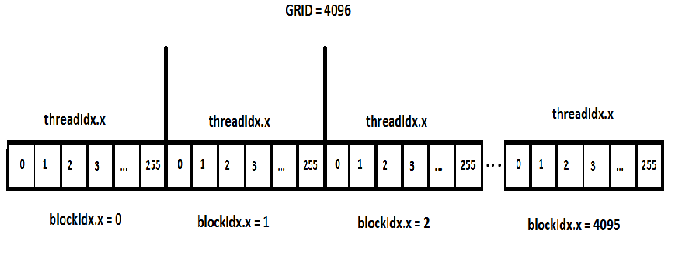
\includegraphics{CUDABlocksAndThreads.png}
\caption{Grid contend. Blocks and threads.}
Source: Own image
\end{figure}
\FloatBarrier

Firstly we have the biggest element which is Grid. 
That element is just entire GPU chip. Nevertheless it is mistake to consider Grid as a single graphics card.
There are Graphics card on the market with a multiple GPUs.
\\
Grid has certain number of blocks. It can be 4096 like in Figure 2.1. 
Blocks are controlled by multiprocessors - MP. One MP can control one block or more, one block in never controlled by multiple processors.
Multiprocessors are divided into stream processors - SP. Stream processor simillar to MP contorll one or more threads in a block.

\section{Detailed GPU data}
Thanks to deviceQueryDrv software provided by Nvidia we can estimate our GPU specification like Total amount of constant memory, max dimension size of a thread block (x,y,z) or maximum number of threads per block etc.\\



\begin{figure}[h!]
\centering
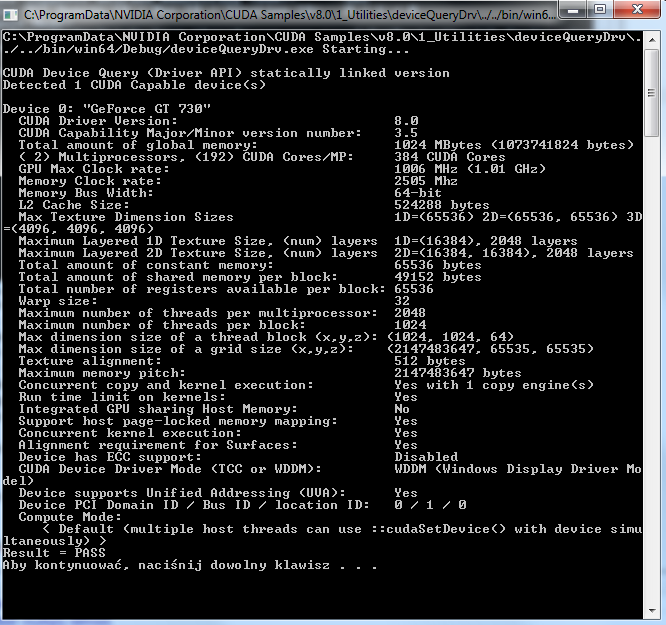
\includegraphics{CUDAParam.PNG}
\caption{Grid contend. Blocks and threads.}
Source: Own image
\end{figure}
\FloatBarrier


Crucial parameter of GPU is warp size. Warp size says about amount of threads which concurrently run on an MP. Threads are running pipelined and parallel. One MP is usually 8 SPs, and one SP can have 4 instruction in pipline. So we have 32 concurrent executed instructions.

\section{Used algorithm}

FOR CSR we have following algorithm:

\begin{lstlisting}[language=C++]

__global__ void CSRCudaMatrixVectorProduct(const int &M, const int * JA, const int * IRP, const double * AS, double * IN, double * OUT)
{
	//Based on local memory
	extern __shared__ double storeArray[];

	unsigned int warpSize = 32; //All modern GPU have warp sizeOfInt 32
	unsigned int threadID = blockIdx.x * blockDim.x + threadIdx.x;
	unsigned int warpID = threadID / warpSize;
	unsigned int threadIndOfWarp = threadID & (warpSize - 1);

	unsigned int threadIndex = threadIdx.x;
	unsigned int selected = warpID;

	if (selected < M)
	{
		unsigned int rowBegining = IRP[selected];
		unsigned int endOfRow = IRP[selected + 1];

		storeArray[threadIdx.x] = 0;
		for (unsigned j = rowBegining + threadIndOfWarp; j < endOfRow; j+= warpSize)
		{
			storeArray[threadIdx.x] += AS[j] * IN[JA[j]];
		
		}


		if (threadIndOfWarp < 16) storeArray[threadIdx.x] += storeArray[threadIdx.x + 16];
		if (threadIndOfWarp < 8) storeArray[threadIdx.x] += storeArray[threadIdx.x + 8];
		if (threadIndOfWarp < 4) storeArray[threadIdx.x] += storeArray[threadIdx.x + 4];
		if (threadIndOfWarp < 2) storeArray[threadIdx.x] += storeArray[threadIdx.x + 2];
		if (threadIndOfWarp < 1) storeArray[threadIdx.x] += storeArray[threadIdx.x + 1];


		if (threadIndOfWarp == 0)
		{
			OUT[selected] = storeArray[threadIdx.x];
		}
	}	
	
}
\end{lstlisting}




That solution involves much more threads into work. For instance simpler solution with one thread per matrix row 
like below:\\\\
\\
For EELPACK storage system there is following CUDA solution:\\

\begin{lstlisting}[language=C++]
__global__ void ELLPackCudaMatrixVectorProduct(const int &M, const int & NZ, const int * JA, const double * AS, double * IN, double * OUT, int & maxBlocks)
{
	//Based on local memory
	extern __shared__ double storeArray[];

	unsigned int block = blockIdx.x;
	unsigned int warpSize = 32;

	while (block < NZ)
	{
		unsigned int threadIndex = threadIdx.x;
		unsigned int threadCompIdx = blockIdx.x * NZ + threadIdx.x;
		//All modern GPU have warp sizeOfInt 32
		unsigned int warpIndex = threadCompIdx / warpSize;
		unsigned int threadIndegOfWarp = threadCompIdx & (warpSize - 1);


		unsigned int limit = blockDim.x / 2;
		storeArray[threadIdx.x] = 0;

		while (threadIndex < NZ)
		{
			storeArray[threadIdx.x] += AS[threadCompIdx] * IN[JA[threadCompIdx]];

			threadIndex += blockDim.x;
			threadCompIdx += blockDim.x;
		}
		__syncthreads();

	
		while (limit > 0)
		{
			if (threadIdx.x < limit)
			{
				storeArray[threadIdx.x] = storeArray[threadIdx.x] + storeArray[threadIdx.x + limit];
			}

			__syncthreads();

			limit = limit / 2;
		}

		if (threadIdx.x == 0)
		{
			OUT[block] = storeArray[0];
		}
		block += maxBlocks;
		
	}


}
\end{lstlisting}

Causes problem of idling many threads. This is the reason why we are not using most of our computation resources.




\chapter{OpenMP}

For CRS OpenMP alghoritm is similiar to CUDA one:\\

\begin{lstlisting}[language=C++]
void OpenMP::OpenMPSolver(ReadMatrixCSR & mat, std::vector<double>& X, std::vector<double>& Y,  int threadsNumber, double & timeToComplete, unsigned int numberOfMatrixXColumn)
{
	int numberOfRows = mat.getN();


	std::chrono::high_resolution_clock::time_point start;
	std::chrono::high_resolution_clock::time_point  end;
	double fullTime = 0.0;
	start = std::chrono::high_resolution_clock::now();

	

	#pragma omp parallel for num_threads(threadsNumber)
	for (int i = 0; i < numberOfMatrixXColumn; ++i)
	{
		for (int index = 0; index < mat.getM(); ++index)
		{
			unsigned int upperBound = mat.getSelectedElementIRP(index + 1);

			for (int k = mat.getIRP().at(index); k < upperBound; ++k)
			{
				Y[index + i * numberOfRows] += mat.getSelectedElementAS(k) * X[mat.getSelectedElementJA(k)+ i * numberOfRows];
			}
		}
	}		

	end = std::chrono::high_resolution_clock::now();
	fullTime = std::chrono::duration_cast<std::chrono::nanoseconds>(end - start).count() / 1000000.0;
	timeToComplete = fullTime;	

}
\end{lstlisting}


And for ELLPack format the following algorithm was used:

\begin{lstlisting}[language=C++]
void OpenMP::OpenMPSolver(ReadMatrixELL & mat, std::vector<double>& X, std::vector<double>& Y, int threadsNumber, double & timeToComplete, unsigned int numberOfMatrixXColumn)
{	

	
std::chrono::high_resolution_clock::time_point start;
std::chrono::high_resolution_clock::time_point  end;
double fullTime = 0.0;
start = std::chrono::high_resolution_clock::now();
int numberOfRows = mat.getM();
int numOfElemsInTheBiggestRow = mat.getNumberOfElementsInTheBiggestRow();
	



#pragma omp parallel for num_threads(threadsNumber)
for (int i = 0; i < numberOfMatrixXColumn; ++i)
{
	for (int outputIndex = 0; outputIndex < numberOfRows; ++outputIndex)
	{
		for (int k = 0; k < numOfElemsInTheBiggestRow; ++k)
		{
			long long inputIndex = outputIndex * numOfElemsInTheBiggestRow + k;
			Y[outputIndex + i * numberOfRows] += mat.getSelectedElementAS(inputIndex) * X[mat.getSelectedElementJA(inputIndex) + i * numberOfRows] ;
		}

	}	

}

end = std::chrono::high_resolution_clock::now();
fullTime = std::chrono::duration_cast<std::chrono::nanoseconds>(end - start).count() / 1000000.0;
timeToComplete = fullTime;


}

\end{lstlisting}

\chapter{Performance measurements}

Performance in all cases was measured in MFLOPS. 
For OpenMP we use maximum number of threads available on our PC which is 4. We are checking performance differences related to number of columns in matrices multiplicated by matrices from the internet.
\\
In CUDA case we perform a sparse matrix-vector product for different runs.
\\
Each test was performed 10 times and results are average of all runs. In CUDA case each set of 10 runs is also in a for loop that iterates thought number of matrix column sizes (2,3,4,8), so 4 times. In CUDA case we have results of run 4 times set 10 runs a sparse matrix-vector product, column numbers don't apply into computations. 
\\
In OpenMP analogically we run 10 runs for average results and that set is run for 4 times for each column. In OpenMP case we applies number of columns to our computation and we check what is the impact of the bigger number of columns for a performance.
\\
\\
\\
\\
\\
\\
\\
\\
\\
\\
\\
\\
\\
\\
\\
\\
\\
\\
\\
\\
\\
\\
\\
\\
\\
\\
\\
\\
\\
\\

%Two images on half page
%\begin{figure}[ht]
%  \centering
 % 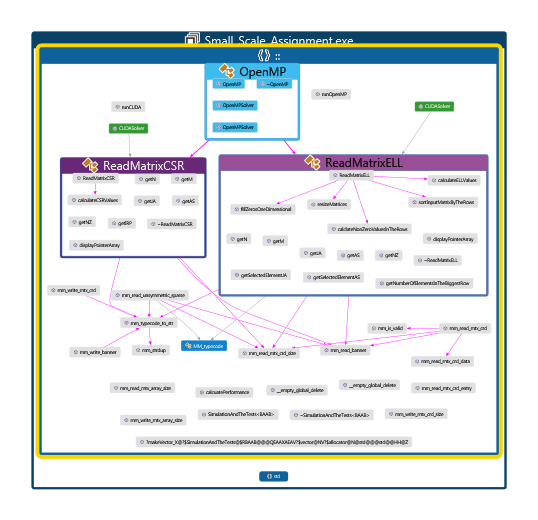
\includegraphics[scale=0.5]{CodeMap.png}
 % \caption{gssr}

%  \vspace*{\floatsep}% https://%tex.stackexchange.com/q/26521/5764

%  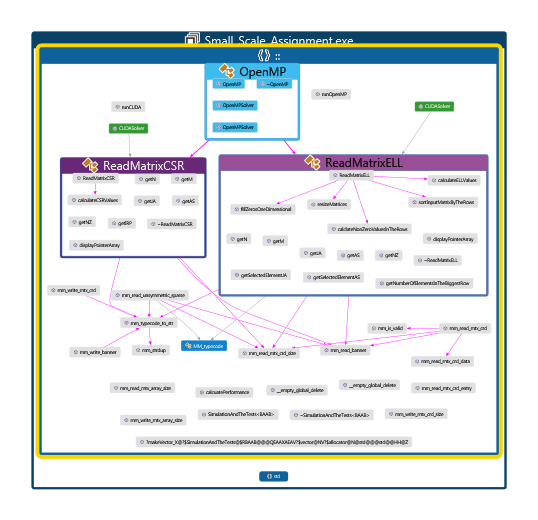
\includegraphics[scale=0.5]{CodeMap.png}
%  \caption{gregre}
%%\end{figure}

\section{cage4.mtx}

\begin{figure}[ht] 
  \label{ fig7} 
  \begin{minipage}[b]{0.5\linewidth}
    \centering
    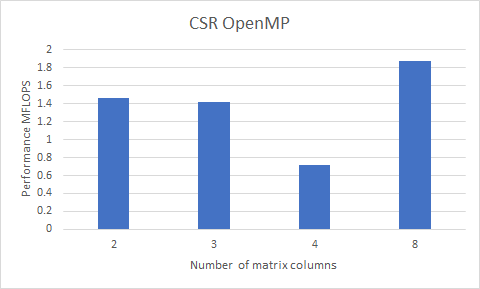
\includegraphics[width=.9\linewidth]{cage4CSRMP.png} 
    \caption{OpenMP CSR results} 
    \vspace{4ex}
  \end{minipage}%%
  \begin{minipage}[b]{0.5\linewidth}
    \centering
    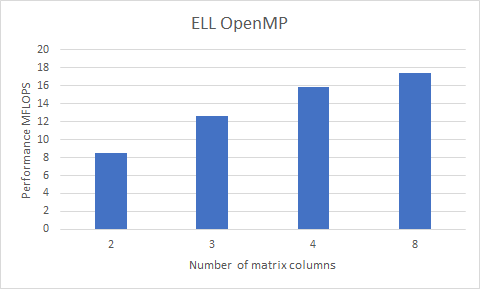
\includegraphics[width=.9\linewidth]{cage4EllMP.png} 
    \caption{OpenMP ELLPack results} 
    \vspace{4ex}
  \end{minipage} 
  \begin{minipage}[b]{0.5\linewidth}
    \centering
    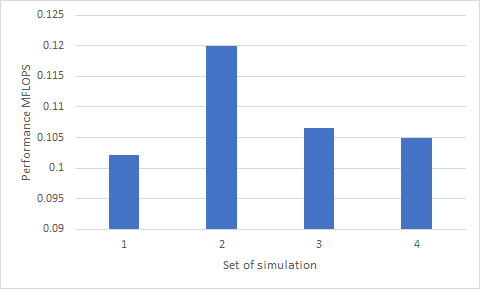
\includegraphics[width=.9\linewidth]{cage4CSRCUDA.png} 
    \caption{CUDA CSR results} 
    \vspace{4ex}
  \end{minipage}%% 
  \begin{minipage}[b]{0.5\linewidth}
    \centering
    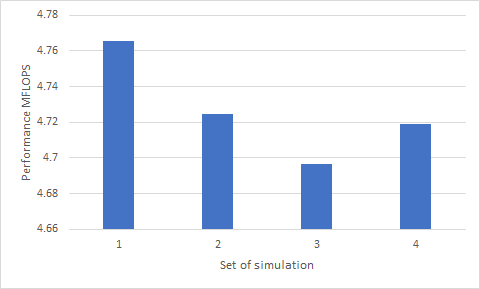
\includegraphics[width=.9\linewidth]{cage4ELLCUDA.png} 
    \caption{CUDA ELLPack  results} 
    \vspace{4ex}
  \end{minipage} 
\end{figure}
\FloatBarrier



\section{adder_dcop_32.mtx}

\begin{figure}[ht] 
  \label{ fig7} 
  \begin{minipage}[b]{0.5\linewidth}
    \centering
    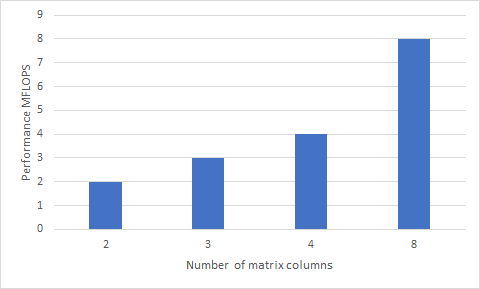
\includegraphics[width=.9\linewidth]{adderCSRMP.png} 
    \caption{OpenMP CSR results} 
    \vspace{4ex}
  \end{minipage}%%
  \begin{minipage}[b]{0.5\linewidth}
    \centering
    \includegraphics[width=.9\linewidth]{adderEllMP.png} 
    \caption{OpenMP ELLPack results} 
    \vspace{4ex}
  \end{minipage} 
  \begin{minipage}[b]{0.5\linewidth}
    \centering
    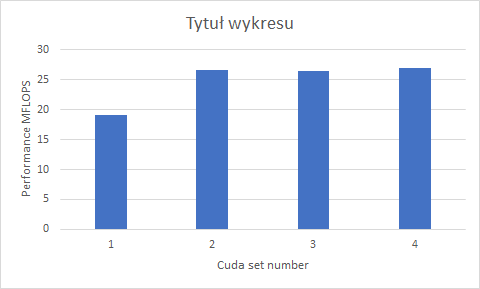
\includegraphics[width=.9\linewidth]{adderCSRCUDA.png} 
    \caption{CUDA CSR results} 
    \vspace{4ex}
  \end{minipage}%% 
  \begin{minipage}[b]{0.5\linewidth}
    \centering
    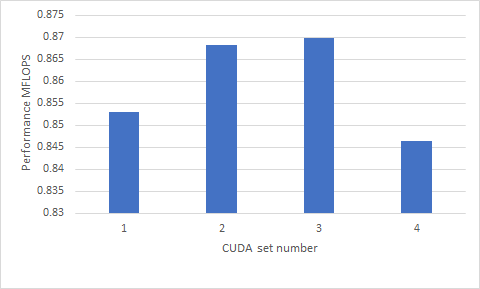
\includegraphics[width=.9\linewidth]{adderELLCUDA.png} 
    \caption{CUDA ELLPack  results} 
    \vspace{4ex}
  \end{minipage} 
\end{figure}
\FloatBarrier


\section{olm1000.mtx}

\begin{figure}[ht] 
  \label{ fig7} 
  \begin{minipage}[b]{0.5\linewidth}
    \centering
    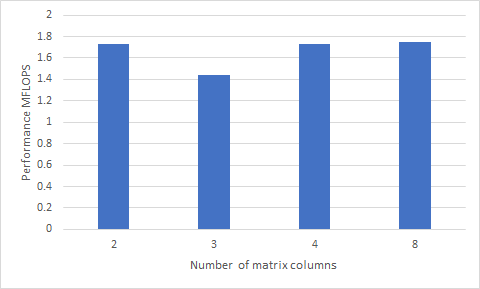
\includegraphics[width=.9\linewidth]{olm100CSRMP.png} 
    \caption{OpenMP CSR results} 
    \vspace{4ex}
  \end{minipage}%%
  \begin{minipage}[b]{0.5\linewidth}
    \centering
    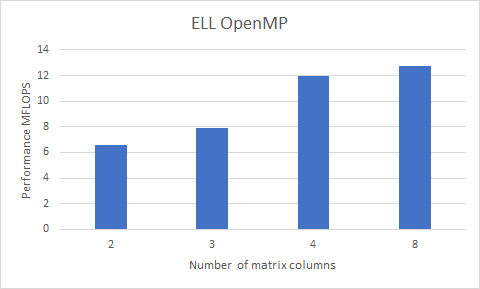
\includegraphics[width=.9\linewidth]{olm100ELLMP.png} 
    \caption{OpenMP ELLPack results} 
    \vspace{4ex}
  \end{minipage} 
  \begin{minipage}[b]{0.5\linewidth}
    \centering
    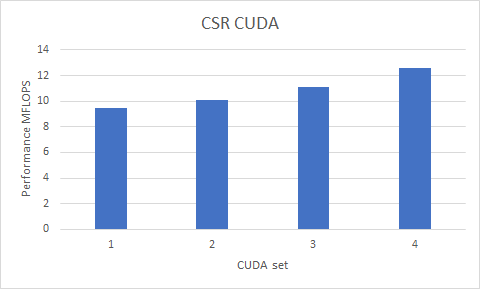
\includegraphics[width=.9\linewidth]{olm100CSRCUDA.png} 
    \caption{CUDA CSR results} 
    \vspace{4ex}
  \end{minipage}%% 
  \begin{minipage}[b]{0.5\linewidth}
    \centering
    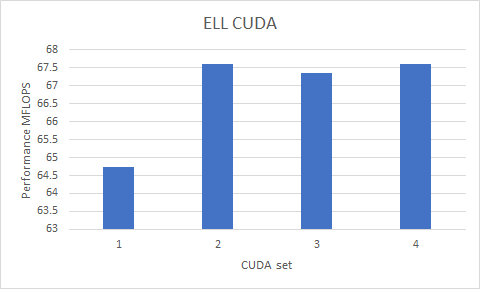
\includegraphics[width=.9\linewidth]{olm100ELLCUDA.png} 
    \caption{CUDA ELLPack  results} 
    \vspace{4ex}
  \end{minipage} 
\end{figure}
\FloatBarrier




\section{mhda416.mtx}

\begin{figure}[ht] 
  \label{ fig7} 
  \begin{minipage}[b]{0.5\linewidth}
    \centering
    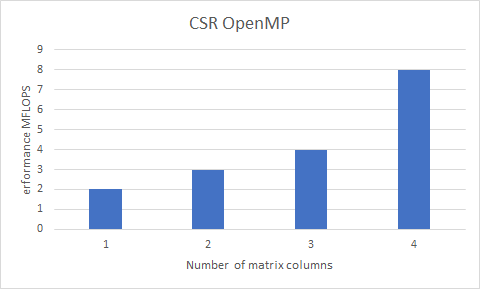
\includegraphics[width=.9\linewidth]{mhda416CSRMP.png} 
    \caption{OpenMP CSR results} 
    \vspace{4ex}
  \end{minipage}%%
  \begin{minipage}[b]{0.5\linewidth}
    \centering
    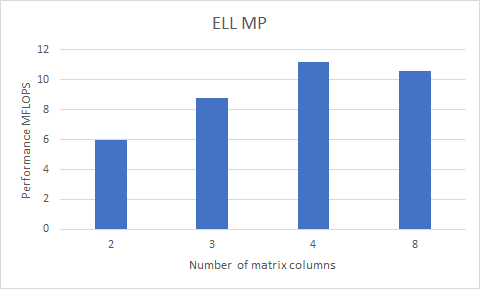
\includegraphics[width=.9\linewidth]{mhda416ELLMP.png} 
    \caption{OpenMP ELLPack results} 
    \vspace{4ex}
  \end{minipage} 
  \begin{minipage}[b]{0.5\linewidth}
    \centering
    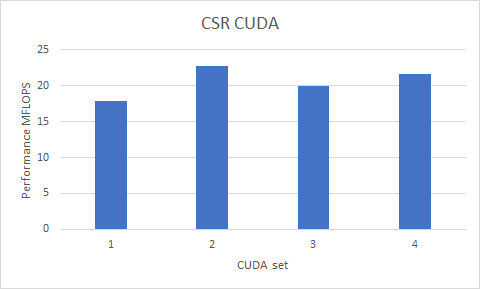
\includegraphics[width=.9\linewidth]{mhda416CSRCUDA.png} 
    \caption{CUDA CSR results} 
    \vspace{4ex}
  \end{minipage}%% 
  \begin{minipage}[b]{0.5\linewidth}
    \centering
    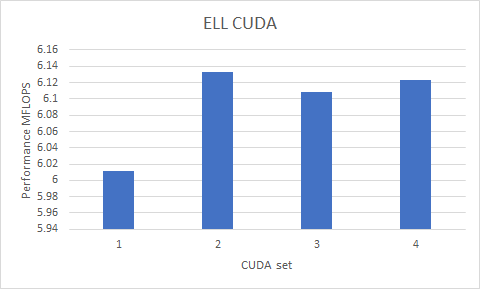
\includegraphics[width=.9\linewidth]{mhda416ELLCUDA.png} 
    \caption{CUDA ELLPack  results} 
    \vspace{4ex}
  \end{minipage} 
\end{figure}
\FloatBarrier



\section{mfce.mtx}

\begin{figure}[ht] 
  \label{ fig7} 
  \begin{minipage}[b]{0.5\linewidth}
    \centering
    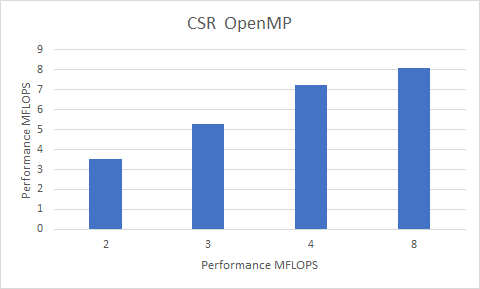
\includegraphics[width=.9\linewidth]{mcfeCSRMP.png} 
    \caption{OpenMP CSR results} 
    \vspace{4ex}
  \end{minipage}%%
  \begin{minipage}[b]{0.5\linewidth}
    \centering
    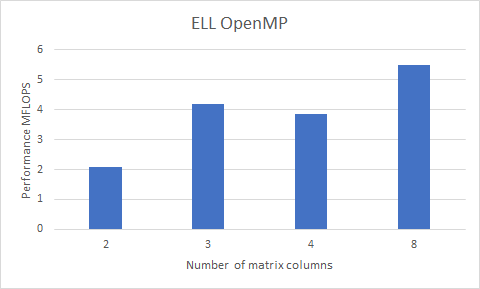
\includegraphics[width=.9\linewidth]{mcfeELLMP.png} 
    \caption{OpenMP ELLPack results} 
    \vspace{4ex}
  \end{minipage} 
  \begin{minipage}[b]{0.5\linewidth}
    \centering
    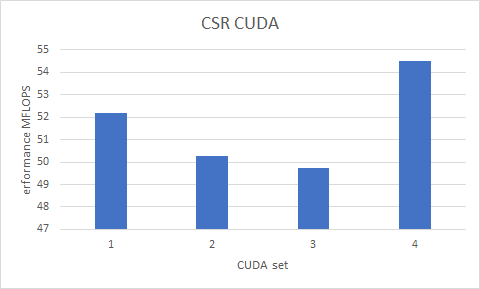
\includegraphics[width=.9\linewidth]{mcfeCSRCUDA.png} 
    \caption{CUDA CSR results} 
    \vspace{4ex}
  \end{minipage}%% 
  \begin{minipage}[b]{0.5\linewidth}
    \centering
    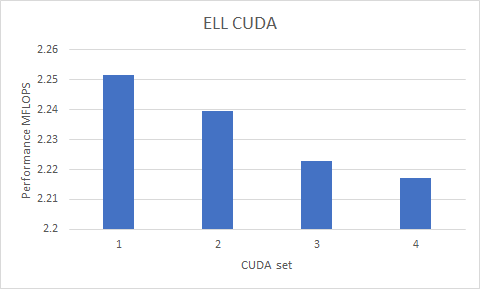
\includegraphics[width=.9\linewidth]{mcfeELLCUDA.png} 
    \caption{CUDA ELLPack  results} 
    \vspace{4ex}
  \end{minipage} 
\end{figure}
\FloatBarrier






\section{rdist2.mtx}

\begin{figure}[ht] 
  \label{ fig7} 
  \begin{minipage}[b]{0.5\linewidth}
    \centering
    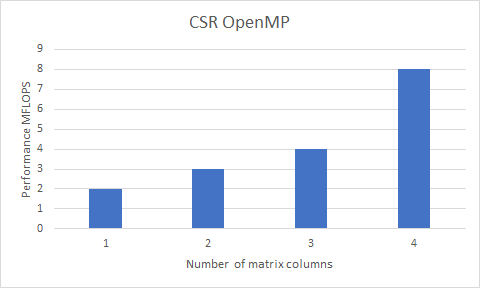
\includegraphics[width=.9\linewidth]{rdist2CSRMP.png} 
    \caption{OpenMP CSR results} 
    \vspace{4ex}
  \end{minipage}%%
  \begin{minipage}[b]{0.5\linewidth}
    \centering
    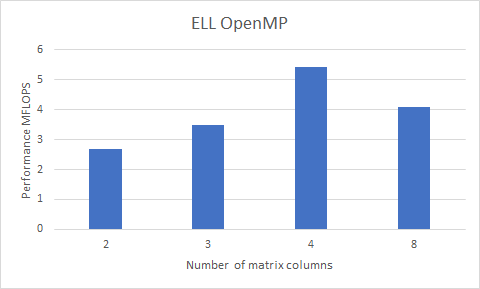
\includegraphics[width=.9\linewidth]{rdist2ELLMP.png} 
    \caption{OpenMP ELLPack results} 
    \vspace{4ex}
  \end{minipage} 
  \begin{minipage}[b]{0.5\linewidth}
    \centering
    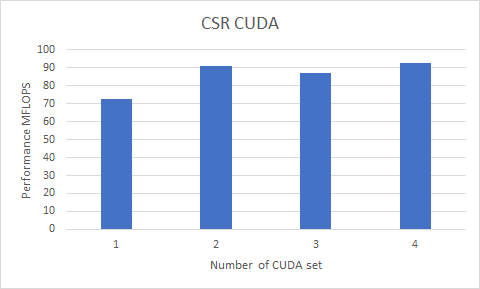
\includegraphics[width=.9\linewidth]{rdist2CSRCUDA.png} 
    \caption{CUDA CSR results} 
    \vspace{4ex}
  \end{minipage}%% 
  \begin{minipage}[b]{0.5\linewidth}
    \centering
    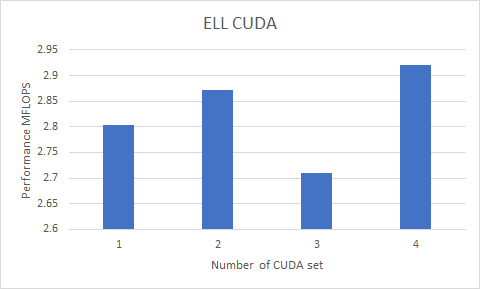
\includegraphics[width=.9\linewidth]{rdist2ELLCUDA.png} 
    \caption{CUDA ELLPack  results} 
    \vspace{4ex}
  \end{minipage} 
\end{figure}
\FloatBarrier




\section{cavity10.mtx}

\begin{figure}[ht] 
  \label{ fig7} 
  \begin{minipage}[b]{0.5\linewidth}
    \centering
    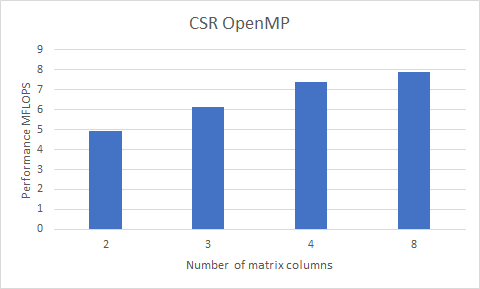
\includegraphics[width=.9\linewidth]{cavity10CSRMP.png} 
    \caption{OpenMP CSR results} 
    \vspace{4ex}
  \end{minipage}%%
  \begin{minipage}[b]{0.5\linewidth}
    \centering
    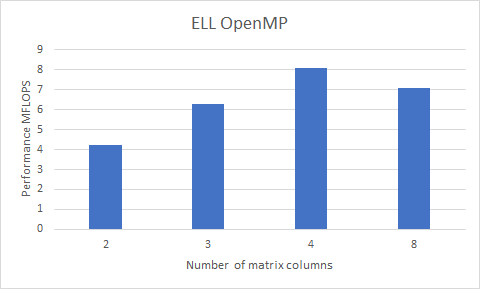
\includegraphics[width=.9\linewidth]{cavity10ELLMP.png} 
    \caption{OpenMP ELLPack results} 
    \vspace{4ex}
  \end{minipage} 
  \begin{minipage}[b]{0.5\linewidth}
    \centering
    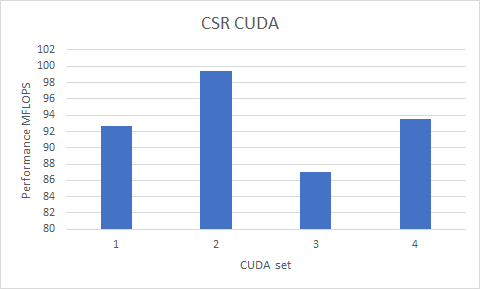
\includegraphics[width=.9\linewidth]{cavity10CSRCUDA.png} 
    \caption{CUDA CSR results} 
    \vspace{4ex}
  \end{minipage}%% 
  \begin{minipage}[b]{0.5\linewidth}
    \centering
    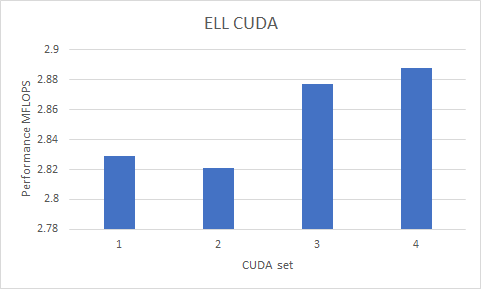
\includegraphics[width=.9\linewidth]{cavity10ELLCUDA.png} 
    \caption{CUDA ELLPack  results} 
    \vspace{4ex}
  \end{minipage} 
\end{figure}
\FloatBarrier



\chapter{Other Nonfunctional Requirements}

\section{Performance Requirements}


\begin{table}[h!]
\centering
\caption{Performance Requirements}
\label{my-label}
\begin{tabular}{|l|l|}
\hline
\multicolumn{2}{|l|}{\textbf{Performance Requirements}}                                                                                                       \\ \hline
Requirement \#: 10     & \begin{tabular}[c]{@{}l@{}}Event/use case \#:-\end{tabular}      \\ \hline

Description:          & \begin{tabular}[c]{@{}l@{}}As efficient solution as possible.\end{tabular}                                                                                                             

\\ \hline
Rationale:            & \begin{tabular}[c]{@{}l@{}} Use as much available computation      \\  resources as possible.\end{tabular}                                                                                                                                                                              \\ \hline
Originator:           & Developer \\ \hline
Fit Criterion:        & \begin{tabular}[c]{@{}l@{}}Windows 7, Nvidia Graphics card, \\ 
Visual Studio 2015 with NSight extension \end{tabular} \\ \hline
Priority:             & 9 \\ \hline
Conflicts             & -                                                                                                                \\ \hline
Supporting Materials: & -                                                                                                                \\ \hline
History:              & Created June, 2017 \\ \hline
\end{tabular}
\end{table}
\FloatBarrier

\begin{table}[h!]
\centering
\caption{Performance Requirements 2}
\label{my-label}
\begin{tabular}{|l|l|}
\hline
\multicolumn{2}{|l|}{\textbf{Performance Requirements 2}}                                                                                                       \\ \hline
Requirement \#: 10     & \begin{tabular}[c]{@{}l@{}}Event/use case \#:-\end{tabular}      \\ \hline

Description:          & \begin{tabular}[c]{@{}l@{}} Good memory managament\end{tabular}                                                                                                             

\\ \hline
Rationale:            & \begin{tabular}[c]{@{}l@{}}To speed up solution and increase\\ the Bandwidth \\ in the future.\end{tabular}                                                                                                                                                                              \\ \hline
Originator:           & Developer \\ \hline
Fit Criterion:        & \begin{tabular}[c]{@{}l@{}} Optimize code using shared memory not \\ only global \end{tabular} \\ \hline
Priority:             & 7 \\ \hline
Conflicts             & -                                                                                                                \\ \hline
Supporting Materials: & -                                                                                                                \\ \hline
History:              & Created June, 2017 \\ \hline
\end{tabular}
\end{table}
\FloatBarrier

\chapter{Conclusions}

Using parallel approach in programming can bring really big performance increase. We have to struggle with many constraints in each parallel solution of specific problem.
During the tests performance we observed that for OpenMP in many case we had a significant performance rise. It was not linear but for instance in cage4.mtx between 2 row and 8 there was approximately 2 times bigger performance for the second case. Not in all the tests we observed performance rise for a bigger number of columns, sometimes like in mhda416.mtx we received lower performance for the 8 columns than for 4.
On our PC generally we achieved much more bigger performance than in OpenMP case, one of the reasons of that fact is only 4 threads old processor (released in 2009) against 384 CUDA cores. Of course in CUDA case we performed matrix-vector calculations, nevertheless in CUDA case performance was sometimes even over 10 times better like in the cavity10.mtx.
\\
\\
 Optimizing parallel code for each different problem is much more challenging comparing to single thread solutions. Developer have to predict many cases and uses many seemingly unusual optimization methods when we think about single thread like loop unrolling. Also it is necessary to have as less idle threads as possible - we want to force in the best case all resources to work.

\chapter{Appendix A}




\begin{lstlisting}[language=C++, caption=main.cu]

#include "cuda_runtime.h"
#include "device_launch_parameters.h"
#include <iostream>
#include <stdio.h>
#include <cstdlib>
#include <vector>
#include <string>
#include "ReadMatrixCSR.h"
#include "ReadMatrixELL.h"
#include "SimulationAndTheTests.h"
#include "SimulationAndTheTests.cpp"

#include <stdlib.h>
#include <stdio.h>
#include <string.h>
#include <cstdlib>
#include <cuda.h>
#include <helper_cuda_drvapi.h>
#include <drvapi_error_string.h>
#include  "deviceQueryDrv.h"



/**
Zmienc nazwu

*/



void displayValues(std::vector<int> JA, std::vector<int> IRP, std::vector<double> AS )
{

	//Output file in to the project folder
	std::ofstream storeArray("output4.txt");
	if (storeArray.is_open())
	{
		storeArray << "JA has folllowing values: ";
		for (std::vector<int>::const_iterator i = JA.begin(); i != JA.end(); ++i)
		{
			storeArray << *i << ' ';
		}

		storeArray << std::endl;

		

		storeArray << "IRP has folllowing values: ";
		for (std::vector<int>::const_iterator i = IRP.begin(); i != IRP.end(); ++i)
		{
			storeArray << *i << ' ';
		}

		storeArray << std::endl;

		storeArray << "AS has folllowing values: ";
		for (std::vector<double>::const_iterator i = AS.begin(); i != AS.end(); ++i)
		{
			storeArray << *i << ' ';
		}

		storeArray << std::endl;

	}

}



void displayOneDimensionalELLValues(std::vector<int> JA, std::vector<double> AS)
{

	//Output file in to the project folder
	std::ofstream storeArray("ELLOneDimesionalNEW.txt");
	if (storeArray.is_open())
	{
		storeArray << "JA has folllowing values: ";
		for (std::vector<int>::const_iterator i = JA.begin(); i != JA.end(); ++i)
		{
			storeArray << *i << ' ';
		}

		storeArray << std::endl;


		storeArray << "AS has the following values: ";
		for (std::vector<double>::const_iterator i = AS.begin(); i != AS.end(); ++i)
		{
			storeArray << *i << ' ';
		}

		storeArray << std::endl;

	}

}

void readCudaParameters()
{
	CUdevice dev;
	int deviceCount = 0;

	// note your project will need to link with cuda.lib files on windows
	printf("CUDA Device Query (Driver API) statically linked version \n");

	CUresult error_id = cuInit(0);

	if (error_id != CUDA_SUCCESS)
	{
		printf("cuInit(0) returned %d\n-> %s\n", error_id, getCudaDrvErrorString(error_id));
		printf("Result = FAIL\n");
		exit(EXIT_FAILURE);
	}

	error_id = cuDeviceGetCount(&deviceCount);

	if (error_id != CUDA_SUCCESS)
	{
		printf("cuDeviceGetCount returned %d\n-> %s\n", (int)error_id, getCudaDrvErrorString(error_id));
		printf("Result = FAIL\n");
		exit(EXIT_FAILURE);
	}

	// This function call returns 0 if there are no CUDA capable devices.
	if (deviceCount == 0)
	{
		printf("There are no available device(s) that support CUDA\n");
	}
	else
	{
		printf("Detected %d CUDA Capable device(s)\n", deviceCount);
	}


	for (dev = 0; dev < deviceCount; ++dev)
	{
		int warpSize;
		getCudaAttribute<int>(&warpSize, CU_DEVICE_ATTRIBUTE_WARP_SIZE, dev);
		std::cout << "Warp size is: " << warpSize << std::endl;
	}

}





int main(int argc, char *argv[])
{

	std::vector<std::string> matriresList;
	std::cout << "USAGE: put all matrices into your main project folder \nor mass one matrix as program parameter\n Program gives .xls files in the output in program main directory folder\n" << std::endl;
	
	std::string currentMattix = argv[1];
	std::cout << "Argument 1 is: " << currentMattix << std::endl;

	readCudaParameters();

	std::vector<std::string> matricesNames = { 	
		"cage4.mtx",
		
		 };


	int simulationRuns = 10;
	unsigned int numberOfThreads = 4;
	unsigned int sizeOfBlock = 64;
	unsigned int maxNumberOfBlocks = 4096;

	std::cout << "The number of simulations repetitions: " << simulationRuns << std::endl << std::endl;;
	/**
	//Start Parallel computation
	*/
	for (auto it : matricesNames)
	{
		// Read input matrices
		ReadMatrixCSR matrixCSR(it);
		ReadMatrixELL matrixELL(it);
		SimulationAndTheTests<ReadMatrixCSR> simCSR;
		SimulationAndTheTests<ReadMatrixELL> simELLPack;
		//std::cout<<"ELL SIZE: "<<sizeof(matrixELL)<<std::endl;

		//OpenMP Run
		simCSR.runOpenMP(matrixCSR, numberOfThreads, simulationRuns);
		simELLPack.runOpenMP(matrixELL, numberOfThreads, simulationRuns);

		//CUDA Run
		simCSR.runCUDA(matrixCSR, numberOfThreads, sizeOfBlock, maxNumberOfBlocks, simulationRuns);
		simELLPack.runCUDA(matrixELL, numberOfThreads, sizeOfBlock, maxNumberOfBlocks, simulationRuns);

	}

	system("pause");
    return 0;
}


\end{lstlisting}


\begin{lstlisting}[language=C++, caption=SimulationAndTheTests.h]

#pragma once
#ifndef _RUNSIMULATION_H_
#define _RUNSIMULATION_H_

#include "ReadMatrixCSR.h"
#include "ReadMatrixELL.h"
#include "CudaSolver.h"
#include "OpenMP.h"
#include <vector>
#include <chrono>
#include <random>
#include <type_traits>

#include <iostream>
#include <stdio.h>
#include <iterator>
#include <string>
#include <memory>
#include <map>
#include <iomanip>


template<class classType>
class SimulationAndTheTests
{
	
	std::vector<int> matricesNumberOfColumns;

public:
	SimulationAndTheTests();
	~SimulationAndTheTests();
	
	auto calcuatePerformance(int NZ, double completionTime);
	/**
	Runs CUDA solution.
	*/
	void runCUDA(classType & mat, int numberOfThreads, int sizeOfBlock, int maximumBlocksdouble, int numberOfSimulationRuns);

	void runOpenMP(classType & mat, int numberOfThreads, int numberOfSimulationRuns);

	/**
	Make an vector for parallel matrix-vector multiplication
	*/
	void makeVector_X(std::vector<double> & X, int sizeOfMaxtixRow, int numberOfMatrixXColumns);
	
	


};



#endif




\end{lstlisting}




\begin{lstlisting}[language=C++, caption=SimulationAndTheTests.cpp]

#include "SimulationAndTheTests.h"


template<class classType>
SimulationAndTheTests<classType>::SimulationAndTheTests()
{
	matricesNumberOfColumns = { 2,3,4,8 };
}

template<class classType>
SimulationAndTheTests<classType>::~SimulationAndTheTests()
{
}



template<class classType>
auto SimulationAndTheTests<classType>::calcuatePerformance(int NZ, double completionTime)
{
	return 2.0 * (float) NZ / completionTime / (float)1000.0;
}

template<class classType>
void SimulationAndTheTests<classType>::runCUDA(classType & mat, int numberOfThreads, int sizeOfBlock, int maximumBlocks, int numberOfSimulationRuns)
{

	std::ofstream results;
	ReadMatrixELL matrixELL1("cage4.mtx");
	OpenMP omp;


	double timeToComplete = 0;
	double avarageTime = 0;
	double avaragePerfomrance = 0;
	double avgTime2 = 0;
	double avaPerfomrance2 = 0;
	std::vector<double> X;
	std::vector<double> Y;

	int NZtimesNumberOfMatrixColumns = mat.getNZ(); // *matricesNumberOfColumns[k];
	X.resize(mat.getNZ()); // X.resize(NZtimesNumberOfMatrixColumns);
	Y.resize(mat.getNZ()); // Y.resize(NZtimesNumberOfMatrixColumns);
	std::fill(X.begin(), X.end(), 1.0);
	std::fill(Y.begin(), Y.end(), 0);


	std::string resultsFileName = (std::string) typeid(classType).name() + "CUDA" + mat.getMatrixName() + ".xls";
	results.open(resultsFileName);
	//In the .xls files next column separator is "\t" in Excel. 
	//When we want to use .csv extension files, depend on system separator could be "," or ";" .
	results << (std::string) typeid(classType).name() + " CUDA" << std::endl;
	results << "Number of matrix columns\t Performance MFLOPS" << std::endl;
	for (int k = 0; k < matricesNumberOfColumns.size(); ++k)
	{
		for (int i = 0; i < numberOfSimulationRuns; ++i)
		{

			std::chrono::high_resolution_clock::time_point start = std::chrono::high_resolution_clock::now();

			//Compute CUDA matrix by "tall" dense matrix multiplication product
			CUDASolver(mat, X, Y, sizeOfBlock, maximumBlocks, timeToComplete);

			std::chrono::high_resolution_clock::time_point end = std::chrono::high_resolution_clock::now();
			double complete = std::chrono::duration_cast<std::chrono::nanoseconds>(end - start).count() / 1000000.0;
			avarageTime += complete;
			avaragePerfomrance += calcuatePerformance(NZtimesNumberOfMatrixColumns, complete);

		}
		avarageTime /= numberOfSimulationRuns;
		avaragePerfomrance /= numberOfSimulationRuns;
		//Save results to the file
		results << matricesNumberOfColumns[k];
		results << "\t" << avaragePerfomrance << "\n";
		avgTime2 += avarageTime;
		avaPerfomrance2 = avaragePerfomrance;
		avarageTime = 0;
		avaragePerfomrance = 0;
	}
	std::cout << "Average CUDA time in milliseconds: " << avgTime2 / matricesNumberOfColumns.size() << " ms\n";
	std::cout << "CUDA average performance is: " << avaPerfomrance2 / matricesNumberOfColumns.size() << " MFLOPS\n" << std::endl;

}




template<class classType>
void SimulationAndTheTests<classType>::runOpenMP(classType &  mat, int numberOfThreads, int numberOfSimulationRuns)
{
	std::ofstream results;
	ReadMatrixELL matrixELL1("cage4.mtx");
	OpenMP omp;
	double timeToComplete = 0;
	std::vector<double> X;
	std::vector<double> Y;
//	makeVector_X(X, mat.getN(), numberOfMatrixXColumns);
	double avarageTime = 0;
	double avaragePerfomrance = 0;
	double avgTime2 = 0;
	double avaPerfomrance2 = 0;

	std::string resultsFileName = (std::string) typeid(classType).name() + "OpenMP" + mat.getMatrixName() + ".xls";
	

	results.open(resultsFileName); 
	results << (std::string) typeid(classType).name() + " OpenMP" << std::endl;
	//In the .xls files next column separator is "\t" in Excel. 
	//When we want to use .csv extension files, depend on system separator could be "," or ";" .
	results << "Number of matrix columns\t Performance MFLOPS" << std::endl;
	
	try
	{
		for (int k = 0; k < matricesNumberOfColumns.size(); ++k)
		{
			int NZtimesNumberOfMatrixColumns = mat.getNZ() * matricesNumberOfColumns[k];
			X.resize(NZtimesNumberOfMatrixColumns);
			Y.resize(NZtimesNumberOfMatrixColumns);
			std::fill(X.begin(), X.end(), 1.0);
			std::fill(Y.begin(), Y.end(), 0);

			for (int i = 0; i < numberOfSimulationRuns; ++i)
			{

				std::chrono::high_resolution_clock::time_point start = std::chrono::high_resolution_clock::now();
				//Compute OpenMP matrix by "tall" dense matrix multiplication product
				omp.OpenMPSolver(mat, X, Y, numberOfThreads, timeToComplete, matricesNumberOfColumns[k]);
				std::chrono::high_resolution_clock::time_point  end = std::chrono::high_resolution_clock::now();
				avarageTime += timeToComplete;
				avaragePerfomrance += calcuatePerformance(NZtimesNumberOfMatrixColumns, timeToComplete);

			}
			//results << "Number of columns " << matricesNumberOfColumns[k] << "\n";
			avarageTime /= numberOfSimulationRuns;
			avaragePerfomrance /= numberOfSimulationRuns;
			results << matricesNumberOfColumns[k];
			results << "\t" << avaragePerfomrance << "\n";
			avgTime2 += avarageTime;
			avaPerfomrance2= avaragePerfomrance;
			avarageTime = 0;
			avaragePerfomrance = 0;
		}


		std::cout << "Average OpenMP time in milliseconds: " << avgTime2 / matricesNumberOfColumns.size() << " ms\n";
		std::cout << "OpenMP average performance is: " << avaPerfomrance2 / matricesNumberOfColumns.size() << " MFLOPS\n" << std::endl;
	}
	catch (std::exception & e)
	{
		std::cout << "Standard exception: " << e.what() << std::endl;
	}


}

template<class classType>
void SimulationAndTheTests<classType>::makeVector_X(std::vector<double>& X, int sizeOfMaxtixRow, int numberOfMatrixXColumns)
{
	//X.resize(sizeOfMaxtixRow * numberOfMatrixXColumns);
	unsigned seed;
	int randNumber;
	
	//for (int i = 0; i < sizeOfMaxtixRow; ++i)
	for (int i = 0; i < sizeOfMaxtixRow * numberOfMatrixXColumns; ++i)
	{
		seed = std::chrono::system_clock::now().time_since_epoch().count();
		std::default_random_engine dre(seed);
		std::uniform_real_distribution<double> gen(0, 5);
		randNumber = gen(dre);
		X[i] = 1.0;
	}

	


}






\end{lstlisting}




\begin{lstlisting}[language=C++, caption=OpenMP.h]


#pragma once
#include "ReadMatrixCSR.h"
#include "ReadMatrixELL.h"
#include <omp.h>
#include <iostream>
#include <vector>
#include <chrono>
#include <random>
#include <type_traits>
class OpenMP
{
public:
	OpenMP();
	~OpenMP();

	void OpenMPSolver(ReadMatrixCSR &mat, std::vector<double> & X, std::vector<double> & Y, int threadsNumber, double & timeToComplete, unsigned int numberOfMatrixXColumn);


	void OpenMPSolver(ReadMatrixELL &mat, std::vector<double> & X, std::vector<double> & Y, int threadsNumber, double & timeToComplete, unsigned int numberOfMatrixXColumn);
};




\end{lstlisting}




\begin{lstlisting}[language=C++, caption=OpenMP.cpp]
#include "OpenMP.h"
#define export OMP_NUM_THREADS = 4

OpenMP::OpenMP()
{
}

OpenMP::~OpenMP()
{
}



void OpenMP::OpenMPSolver(ReadMatrixCSR & mat, std::vector<double>& X, std::vector<double>& Y,  int threadsNumber, double & timeToComplete, unsigned int numberOfMatrixXColumn)
{
	int numberOfRows = mat.getN();


	std::chrono::high_resolution_clock::time_point start;
	std::chrono::high_resolution_clock::time_point  end;
	double fullTime = 0.0;
	start = std::chrono::high_resolution_clock::now();

	

	#pragma omp parallel for num_threads(threadsNumber)
	for (int i = 0; i < numberOfMatrixXColumn; ++i)
	{
		for (int index = 0; index < mat.getM(); ++index)
		{
			unsigned int upperBound = mat.getSelectedElementIRP(index + 1);

			for (int k = mat.getIRP().at(index); k < upperBound; ++k)
			{
				Y[index + i * numberOfRows] += mat.getSelectedElementAS(k) * X[mat.getSelectedElementJA(k)+ i * numberOfRows];
			}
		}
	}		

	end = std::chrono::high_resolution_clock::now();
	fullTime = std::chrono::duration_cast<std::chrono::nanoseconds>(end - start).count() / 1000000.0;
	timeToComplete = fullTime;	

}




void OpenMP::OpenMPSolver(ReadMatrixELL & mat, std::vector<double>& X, std::vector<double>& Y, int threadsNumber, double & timeToComplete, unsigned int numberOfMatrixXColumn)
{	

	
std::chrono::high_resolution_clock::time_point start;
std::chrono::high_resolution_clock::time_point  end;
double fullTime = 0.0;
start = std::chrono::high_resolution_clock::now();
int numberOfRows = mat.getM();
int numOfElemsInTheBiggestRow = mat.getNumberOfElementsInTheBiggestRow();
	



#pragma omp parallel for num_threads(threadsNumber)
for (int i = 0; i < numberOfMatrixXColumn; ++i)
{
	for (int outputIndex = 0; outputIndex < numberOfRows; ++outputIndex)
	{
		for (int k = 0; k < numOfElemsInTheBiggestRow; ++k)
		{
			long long inputIndex = outputIndex * numOfElemsInTheBiggestRow + k;
			Y[outputIndex + i * numberOfRows] += mat.getSelectedElementAS(inputIndex) * X[mat.getSelectedElementJA(inputIndex) + i * numberOfRows] ;
		}

	}	

}

end = std::chrono::high_resolution_clock::now();
fullTime = std::chrono::duration_cast<std::chrono::nanoseconds>(end - start).count() / 1000000.0;
timeToComplete = fullTime;


}







\end{lstlisting}




\begin{lstlisting}[language=C++, caption=ReadMatrixCSR.h]

#pragma once
#include <stdio.h>
#include <stdlib.h>
#include <string>
#include "mmio.h"
#include <iostream>
#include <vector>
#include <algorithm>
#include <fstream>
#include <tuple>
#include <memory>


class ReadMatrixCSR
{

private:

	
	int M, N, nz;
	int i;
	
	std::string matrixName;
	//int * JA;
	//double * AS;
	//int * IRP; // Pointer to IRP array

	std::unique_ptr<int[]>  JA;
	std::unique_ptr<double[]>  AS;
	std::unique_ptr<int[]>  IRP;

	std::vector<double> asVector;
	std::vector<int> jaVector;
	std::vector<int> irpVector;

	//std::vector<std::pair<int, double> > rowsAndValues;


	void calculateCSRValues(std::vector<std::tuple<int, int, double> > rowsAndValues, int * J);

	void displayPointerArray(int * arr);

	

public:	

	ReadMatrixCSR(std::string matrixName);
	ReadMatrixCSR(const ReadMatrixCSR& copy);
	~ReadMatrixCSR();
	std::vector<int> getIRP();
	std::vector<double> getAS();
	std::vector<int> getJA();
	double getSelectedElementAS(int elemIndex) const;
	int getSelectedElementJA(int elemIndex) const;
	int getSelectedElementIRP(int elemIndex) const;
	int getM();
	int getNZ();
	int getN();
	std::string getMatrixName();

};





\end{lstlisting}




\begin{lstlisting}[language=C++, caption=ReadMatrixCSR.cpp]

#include "ReadMatrixCSR.h"




ReadMatrixCSR::ReadMatrixCSR(std::string matrixName)
{
	(*this).matrixName = matrixName;
	MM_typecode matcode;
	FILE *f;
	int  *I, *J;
	int ret_code;
	double *matrixValue;


	std::vector<std::tuple<int, int, double> > rowsAndValues;

	if ((f = fopen(matrixName.c_str(), "r")) == NULL)
	{
		std::cout << "There is no matrix to read" << std::endl;
		exit(1);
	}
			

	if (mm_read_banner(f, &matcode) != 0)
	{
		printf("Could not process Matrix Market banner.\n");
		exit(1);
	}


	/*  This is how one can screen matrix types if their application */
	/*  only supports a subset of the Matrix Market storeArray types.      */

	if (mm_is_complex(matcode) && mm_is_matrix(matcode) &&
		mm_is_sparse(matcode))
	{
		printf("Sorry, this application does not support ");
		printf("Market Market type: [%s]\n", mm_typecode_to_str(matcode));
		exit(1);
	}

	/* find out size of sparse matrix .... */

	if ((ret_code = mm_read_mtx_crd_size(f, &M, &N, &nz)) != 0)
		exit(1);


	/* reseve memory for matrices */

	I = (int *)malloc(nz * sizeof(int));
	J = (int *)malloc(nz * sizeof(int));
	matrixValue = (double *)malloc(nz * sizeof(double));


	/* NOTE: when reading in doubles, ANSI C requires the use of the "l"  */
	/*   specifier as in "%lg", "%lf", "%le", otherwise errors will occur */
	/*  (ANSI C X3.159-1989, Sec. 4.9.6.2, p. 136 lines 13-15)            */


	
	for (i = 0; i<nz; i++)
	{
		fscanf(f, "%d %d %lg\n", &I[i], &J[i], &matrixValue[i]);
		I[i]--;  /* adjust from 1-based to 0-based */
		J[i]--;
	}

	if (f != stdin) fclose(f);

	(*this).JA = std::make_unique<int[]>(nz);
	(*this).IRP = std::make_unique<int[]>(M + 1);
	(*this).AS = std::make_unique<double[]>(nz);
	(*this).IRP[0] = 0;
	(*this).IRP[M] = nz;

	std::cout << "This matrix has " << N << " rows " << M << " columns and  " << nz <<" non zero values " << std::endl;

	rowsAndValues.resize(nz);
	for (int i = 0; i < nz; ++i)
	{
		rowsAndValues[i] = std::make_tuple(I[i], J[i], matrixValue[i]);
		
	}

	//Lambda sorting
	std::sort(rowsAndValues.begin(), rowsAndValues.end(), []( auto const &left, auto const &right) {
		if (std::get<0>(left) < std::get<0>(right))
			return true;
		else if ( (std::get<0>(left) == std::get<0>(right)) && (std::get<1>(left) < std::get<1>(right)) )
			return true;
		else
			return false;
						
	});

	calculateCSRValues(rowsAndValues, J);

	for (int i = 0; i < nz; ++i)
	{
		jaVector.push_back(JA.get()[i]);
	}

	for (int i = 0; i < nz; ++i)
	{
		asVector.push_back(AS.get()[i]);
	}

	for (int i = 0; i < M + 1; ++i)
	{
		irpVector.push_back(IRP.get()[i]);
	}

}

ReadMatrixCSR::ReadMatrixCSR(const ReadMatrixCSR & copy)
{

	M = copy.M;
	N = copy.N;
	nz = copy.nz;
	matrixName = copy.matrixName;


	(*this).JA = std::make_unique<int[]>(nz);
	(*this).AS= std::make_unique<double[]>(nz);
	(*this).IRP = std::make_unique<int[]>(M + 1);
	irpVector = copy.irpVector;
	asVector = copy.asVector;
	jaVector = copy.jaVector;

	for (int i = 0; i < nz; ++i)
	{
		JA.get()[i] = copy.JA.get()[i];
	}

	for (int i = 0; i < nz; ++i)
	{
		AS.get()[i] = copy.AS.get()[i];
	}

	for (int i = 0; i < M + 1; ++i)
	{
		IRP.get()[i] = copy.IRP.get()[i];
	}

}


void ReadMatrixCSR::calculateCSRValues(std::vector<std::tuple<int, int, double> > rowsAndValues,int * J)
{
	
	int IRPValue = 0;
	int IRPPos = 0;
	
	int columnNumber = J[0];

	for (int i = 0; i < nz; ++i)
	{
		//Create AS vector
		AS[i] = std::get<2>(rowsAndValues[i]);

		//Create JA vector
		JA[i] = std::get<1>(rowsAndValues[i]);

		//Create IRP vector
		if (std::get<0>(rowsAndValues[i]) == IRPPos)
		{
			IRPValue++;
		}
		else
		{
			IRPPos++;
			IRP[IRPPos] = IRPValue;	
			while (std::get<0>(rowsAndValues[i]) != IRPPos)
			{
				IRPPos++;
				IRP[IRPPos] = IRPValue;
			}
		IRPValue++;
		}
	}


}

void ReadMatrixCSR::displayPointerArray(int * arr)
{
	for (int i = 0; i < nz; i++) {

		std::cout << *(arr + i) << " ";
	}
	std::cout << std::endl;
}

std::vector<int> ReadMatrixCSR::getIRP()
{
	return irpVector;
}

std::vector<double> ReadMatrixCSR::getAS()
{

	return  asVector;
}

std::vector<int> ReadMatrixCSR::getJA()
{

	return jaVector;
}

double ReadMatrixCSR::getSelectedElementAS(int elemIndex) const
{
	return AS[elemIndex];
}

int ReadMatrixCSR::getSelectedElementJA(int elemIndex) const
{
	return JA[elemIndex];
}

int ReadMatrixCSR::getSelectedElementIRP(int elemIndex) const
{
	return IRP[elemIndex];
}



int ReadMatrixCSR::getM()
{
	return M;
}

int ReadMatrixCSR::getNZ()
{
	return nz;
}

int ReadMatrixCSR::getN()
{
	return N;
}

std::string ReadMatrixCSR::getMatrixName()
{
	return matrixName;
}







ReadMatrixCSR::~ReadMatrixCSR()
{
	
}


\end{lstlisting}



\begin{lstlisting}[language=C++, caption=ReadMatrixELL.h]

#pragma once
#include <stdio.h>
#include <stdlib.h>
#include <string>
#include "mmio.h"
#include <iostream>
#include <vector>
#include <algorithm>
#include <fstream>
#include <tuple>
#include <memory>

class ReadMatrixELL
{


	private:	
		// M - Rows, N - Columns , Nz - non zero values
		int M, N, nz;
		int numOfElementsInTheBiggestRow;
		std::string matrixName;
		std::unique_ptr<int[]>  JAOneDimensional;
		std::unique_ptr<double[]>  ASOneDimensional;
		std::vector<double> asVector;
		std::vector<int> jaVector;
		//int * JAOneDimensional;
		//double * ASOneDimensional;

		//std::vector<int> nonZeroValuesInTheRows;
		int nonZeroValuesInTheAllRows;

		void resizeMatrices(std::vector<std::tuple<int, int, double> > & rowsAndValues);

		void sortInputMatrixByTheRows(std::vector<std::tuple<int, int, double> > & rowsAndValues);


		
		void calculateELLValues(std::vector<std::tuple<int, int, double> > & rowsAndValues, std::vector<int> & nonZeroValuesInTheRows);


		//Calculates noon zeros in selected row
		void calclateNonZeroValuesInTheRows(std::vector<std::tuple<int, int, double> > & rowsAndValues, std::vector<int> & nonZeroValuesInTheRows);
	

		//Preparing one-dimensional matrix fling it with zeros
		void fillZerosOneDimensional();


		template<typename TYPE>
		void saveOneDimensionalELLMatrix(TYPE * matrix, std::string name, std::vector<int> & nonZeroValuesInTheRows);

		void displayPointerArray(int * arr);



	public:

		ReadMatrixELL(std::string matrixName);
		ReadMatrixELL::ReadMatrixELL(const ReadMatrixELL& copy);
		~ReadMatrixELL();
		std::vector<double> getAS();
		std::vector<int> getJA();
		int getM();
		int getNZ();
		int getN();
		int getNumberOfElementsInTheBiggestRow();
		double getSelectedElementAS(int elemIndex) const;
		int getSelectedElementJA(int elemIndex) const;
		std::string getMatrixName();




};





\end{lstlisting}



\begin{lstlisting}[language=C++, caption=ReadMatrixELL.cpp]


#include "ReadMatrixELL.h"




ReadMatrixELL::ReadMatrixELL(std::string matrixName)
{
	(*this).matrixName = matrixName;

	MM_typecode matcode;
	FILE *f;
	int  *I, *J;
	int ret_code;
	double *matrixValue;
	std::vector<int> nonZeroValuesInTheRows;
	std::vector<std::tuple<int, int, double> > rowsAndValues;

	if ((f = fopen(matrixName.c_str(), "r")) == NULL)
	{
		std::cout << "There is no matrix to read" << std::endl;
		exit(1);
	}


	if (mm_read_banner(f, &matcode) != 0)
	{
		printf("Could not process Matrix Market banner.\n");
		exit(1);
	}


	/*  This is how one can screen matrix types if their application */
	/*  only supports a subset of the Matrix Market storeArray types.      */

	if (mm_is_complex(matcode) && mm_is_matrix(matcode) &&
		mm_is_sparse(matcode))
	{
		printf("Sorry, this application does not support ");
		printf("Market Market type: [%s]\n", mm_typecode_to_str(matcode));
		exit(1);
	}

	/* find out size of sparse matrix .... */

	if ((ret_code = mm_read_mtx_crd_size(f, &M, &N, &nz)) != 0)
		exit(1);


	/* reseve memory for matrices */

	I = (int *)malloc(nz * sizeof(int));
	J = (int *)malloc(nz * sizeof(int));
	matrixValue = (double *)malloc(nz * sizeof(double));


	/* NOTE: when reading in doubles, ANSI C requires the use of the "l"  */
	/*   specifier as in "%lg", "%lf", "%le", otherwise errors will occur */
	/*  (ANSI C X3.159-1989, Sec. 4.9.6.2, p. 136 lines 13-15)            */


	
	for (int i = 0; i<nz; i++)
	{
		fscanf(f, "%d %d %lg\n", &I[i], &J[i], &matrixValue[i]);
		I[i]--;  /* adjust from 1-based to 0-based */
		J[i]--;
	}

	if (f != stdin) fclose(f);



	resizeMatrices(rowsAndValues);


	for (int i = 0; i < nz; ++i)
	{
		rowsAndValues[i] = std::make_tuple(I[i], J[i], matrixValue[i]);

	}

	sortInputMatrixByTheRows(rowsAndValues);
	calclateNonZeroValuesInTheRows(rowsAndValues, nonZeroValuesInTheRows);
	//fillZeros<int>(nonZeroValuesInTheRows);
	fillZerosOneDimensional();
	calculateELLValues(rowsAndValues, nonZeroValuesInTheRows);

	for (int i = 0; i < nonZeroValuesInTheAllRows * numOfElementsInTheBiggestRow; ++i)
	{
		asVector.push_back(ASOneDimensional.get()[i]);
	}

	for (int i = 0; i < nonZeroValuesInTheAllRows * numOfElementsInTheBiggestRow; ++i)
	{
		jaVector.push_back(JAOneDimensional.get()[i]);
	}

}


void ReadMatrixELL::resizeMatrices(std::vector<std::tuple<int, int, double> > & rowsAndValues)
{

	/*
	//Resize JA and AS	two dimensional//
	(*this).JA = new int*[M];
	(*this).AS = new double*[M];
	for (int i = 0; i < N; ++i)
	{
		JA[i] = new int[N];
		AS[i] = new double[N];
	}
	*/
	
	
	rowsAndValues.resize(nz);
	//Resize one dimensional
	long long vectorSize = static_cast<long long>(M) * static_cast<long long>(nz);
	(*this).JAOneDimensional = std::make_unique<int[]>(vectorSize); //new int[vectorSize];
	(*this).ASOneDimensional = std::make_unique<double[]>(vectorSize);
	/*(*this).JAOneDimensional = new int[vectorSize];
	(*this).ASOneDimensional = new double[vectorSize];*/

}


/*
Copy constructor
*/

ReadMatrixELL::ReadMatrixELL(const ReadMatrixELL& copy)
{
	M = copy.M;
	N = copy.N;
	nz = copy.nz;
	numOfElementsInTheBiggestRow = copy.numOfElementsInTheBiggestRow;
	matrixName = copy.matrixName;
	nonZeroValuesInTheAllRows = copy.nonZeroValuesInTheAllRows;
	jaVector = copy.jaVector;
	asVector = copy.asVector;


	long long vectorSize = static_cast<long long>(M) * static_cast<long long>(nz);
	(*this).JAOneDimensional = std::make_unique<int[]>(vectorSize); 
	(*this).ASOneDimensional = std::make_unique<double[]>(vectorSize);
	
	for (int i = 0; i < vectorSize; ++i)
	{
		JAOneDimensional.get()[i] = copy.JAOneDimensional.get()[i];
	}
	
	for (int i = 0; i < vectorSize; ++i)
	{
		ASOneDimensional.get()[i] = copy.ASOneDimensional.get()[i];
	}

}


void ReadMatrixELL::sortInputMatrixByTheRows(std::vector<std::tuple<int, int, double> > & rowsAndValues)
{

	//Lambda sorting
	std::sort(rowsAndValues.begin(), rowsAndValues.end(), [](auto const &left, auto const &right) {
		if (std::get<0>(left) < std::get<0>(right))
			return true;
		else if ((std::get<0>(left) == std::get<0>(right)) && (std::get<1>(left) < std::get<1>(right)))
			return true;
		else
			return false;

	});
}







void ReadMatrixELL::calclateNonZeroValuesInTheRows(std::vector<std::tuple<int, int, double> > & rowsAndValues, std::vector<int> & nonZeroValuesInTheRows)
{
	int nonZeroValuesInThisRow = 0;
	nonZeroValuesInTheRows.resize(N);
	int k = 0;
	int i = 0;

	while (i < nz - 1)
	{

		//Checking if number of row hasn't changed, This won't get last row
		if (std::get<0>(rowsAndValues[i]) == std::get<0>(rowsAndValues[i + 1]))
		{

			++nonZeroValuesInThisRow;
			++i;

		}
		else
		{
			++nonZeroValuesInThisRow; //
			nonZeroValuesInTheRows[k] = nonZeroValuesInThisRow;
			nonZeroValuesInThisRow = 0;
			++k;
			++i;


		}

	}

	//Add number of values to last row
	nonZeroValuesInTheRows[k] = nonZeroValuesInThisRow + 1;


	numOfElementsInTheBiggestRow = *std::max_element(nonZeroValuesInTheRows.begin(), nonZeroValuesInTheRows.end());
	nonZeroValuesInTheAllRows = nonZeroValuesInTheRows.size();

}


void ReadMatrixELL::fillZerosOneDimensional()
{
	long long vectorSize = static_cast<long long>(M) * static_cast<long long>(nz);
	for (long long i = 0; i < vectorSize; ++i)
	{
		ASOneDimensional[i] = 0;
		JAOneDimensional[i] = 0;
	}
}





void ReadMatrixELL::calculateELLValues(std::vector<std::tuple<int, int, double>>& rowsAndValues, std::vector<int>& nonZeroValuesInTheRows)
{
	int nzValueCounter = 0;
	long long idx = 0;
	for (int i = 0; i < nonZeroValuesInTheRows.size(); ++i)
	{
		for (int j = 0; j < nonZeroValuesInTheRows[i]; ++j)
		{

			//One dimensional case
			idx = i * static_cast<long long>(numOfElementsInTheBiggestRow) + j;
			ASOneDimensional[idx] = std::get<2>(rowsAndValues[nzValueCounter]);
			//Store results in C++ style, add one if you want to get Matlab one
			JAOneDimensional[idx] = std::get<1>(rowsAndValues[nzValueCounter]);

			nzValueCounter++;
		}

	}
}


//displaying 1D matrix
template<typename TYPE>
void ReadMatrixELL::saveOneDimensionalELLMatrix(TYPE * matrix, std::string name, std::vector<int> & nonZeroValuesInTheRows)
{
	std::ofstream storeArray(name + " ELLONEDIMENSIONAL.txt");
		storeArray << name << std::endl;
		long long idx = 0;
	//save to file one-dimensional AS or JA
	for (int i = 0; i < nonZeroValuesInTheRows.size(); ++i)
	{
		for (int j = 0; j < numOfElementsInTheBiggestRow; ++j)
		{
			idx = i * static_cast<long long>(numOfElementsInTheBiggestRow) + j;
			storeArray << matrix[idx]<< " ";
		}
		storeArray << std::endl;

	}
	storeArray << std::endl;
	storeArray << std::endl;

}

void ReadMatrixELL::displayPointerArray(int * arr)
{
	for (int i = 0; i < nz; i++) {

		std::cout << *(arr + i) << " ";
	}
	std::cout << std::endl;
}


std::vector<double> ReadMatrixELL::getAS()
{
	return  asVector;
}

std::vector<int> ReadMatrixELL::getJA()
{

	return jaVector;
}

int ReadMatrixELL::getM()
{

	return M;
}

int ReadMatrixELL::getNZ()
{
	return nz;
}

int ReadMatrixELL::getN()
{
	return N;
}

int ReadMatrixELL::getNumberOfElementsInTheBiggestRow()
{
	return numOfElementsInTheBiggestRow;
}

double ReadMatrixELL::getSelectedElementAS(int elemIndex) const
{
	if ((elemIndex > numOfElementsInTheBiggestRow * M) || (elemIndex < 0))
	{
		std::cout << "Out of scope" << std::endl;
		throw std::exception("Out of scope");
	}
	return ASOneDimensional[elemIndex];
}

int ReadMatrixELL::getSelectedElementJA(int elemIndex) const
{
	if ( (elemIndex > numOfElementsInTheBiggestRow * M) || (elemIndex < 0) )
	{
		std::cout << "Out of scope" << std::endl;
		throw std::exception("Out of scope");
	}
	return JAOneDimensional[elemIndex];
}

std::string ReadMatrixELL::getMatrixName()
{
	return matrixName;
}




ReadMatrixELL::~ReadMatrixELL()
{

	
}




\end{lstlisting}





\begin{lstlisting}[language=C++, caption=CudaSolver.h]

#include "ReadMatrixELL.h"




ReadMatrixELL::ReadMatrixELL(std::string matrixName)
{
	(*this).matrixName = matrixName;

	MM_typecode matcode;
	FILE *f;
	int  *I, *J;
	int ret_code;
	double *matrixValue;
	std::vector<int> nonZeroValuesInTheRows;
	std::vector<std::tuple<int, int, double> > rowsAndValues;

	if ((f = fopen(matrixName.c_str(), "r")) == NULL)
	{
		std::cout << "There is no matrix to read" << std::endl;
		exit(1);
	}


	if (mm_read_banner(f, &matcode) != 0)
	{
		printf("Could not process Matrix Market banner.\n");
		exit(1);
	}


	/*  This is how one can screen matrix types if their application */
	/*  only supports a subset of the Matrix Market storeArray types.      */

	if (mm_is_complex(matcode) && mm_is_matrix(matcode) &&
		mm_is_sparse(matcode))
	{
		printf("Sorry, this application does not support ");
		printf("Market Market type: [%s]\n", mm_typecode_to_str(matcode));
		exit(1);
	}

	/* find out size of sparse matrix .... */

	if ((ret_code = mm_read_mtx_crd_size(f, &M, &N, &nz)) != 0)
		exit(1);


	/* reseve memory for matrices */

	I = (int *)malloc(nz * sizeof(int));
	J = (int *)malloc(nz * sizeof(int));
	matrixValue = (double *)malloc(nz * sizeof(double));


	/* NOTE: when reading in doubles, ANSI C requires the use of the "l"  */
	/*   specifier as in "%lg", "%lf", "%le", otherwise errors will occur */
	/*  (ANSI C X3.159-1989, Sec. 4.9.6.2, p. 136 lines 13-15)            */


	
	for (int i = 0; i<nz; i++)
	{
		fscanf(f, "%d %d %lg\n", &I[i], &J[i], &matrixValue[i]);
		I[i]--;  /* adjust from 1-based to 0-based */
		J[i]--;
	}

	if (f != stdin) fclose(f);



	resizeMatrices(rowsAndValues);


	for (int i = 0; i < nz; ++i)
	{
		rowsAndValues[i] = std::make_tuple(I[i], J[i], matrixValue[i]);

	}

	sortInputMatrixByTheRows(rowsAndValues);
	calclateNonZeroValuesInTheRows(rowsAndValues, nonZeroValuesInTheRows);
	//fillZeros<int>(nonZeroValuesInTheRows);
	fillZerosOneDimensional();
	calculateELLValues(rowsAndValues, nonZeroValuesInTheRows);

	for (int i = 0; i < nonZeroValuesInTheAllRows * numOfElementsInTheBiggestRow; ++i)
	{
		asVector.push_back(ASOneDimensional.get()[i]);
	}

	for (int i = 0; i < nonZeroValuesInTheAllRows * numOfElementsInTheBiggestRow; ++i)
	{
		jaVector.push_back(JAOneDimensional.get()[i]);
	}

}


void ReadMatrixELL::resizeMatrices(std::vector<std::tuple<int, int, double> > & rowsAndValues)
{

	/*
	//Resize JA and AS	two dimensional//
	(*this).JA = new int*[M];
	(*this).AS = new double*[M];
	for (int i = 0; i < N; ++i)
	{
		JA[i] = new int[N];
		AS[i] = new double[N];
	}
	*/
	
	
	rowsAndValues.resize(nz);
	//Resize one dimensional
	long long vectorSize = static_cast<long long>(M) * static_cast<long long>(nz);
	(*this).JAOneDimensional = std::make_unique<int[]>(vectorSize); //new int[vectorSize];
	(*this).ASOneDimensional = std::make_unique<double[]>(vectorSize);
	/*(*this).JAOneDimensional = new int[vectorSize];
	(*this).ASOneDimensional = new double[vectorSize];*/

}


/*
Copy constructor
*/

ReadMatrixELL::ReadMatrixELL(const ReadMatrixELL& copy)
{
	M = copy.M;
	N = copy.N;
	nz = copy.nz;
	numOfElementsInTheBiggestRow = copy.numOfElementsInTheBiggestRow;
	matrixName = copy.matrixName;
	nonZeroValuesInTheAllRows = copy.nonZeroValuesInTheAllRows;
	jaVector = copy.jaVector;
	asVector = copy.asVector;


	long long vectorSize = static_cast<long long>(M) * static_cast<long long>(nz);
	(*this).JAOneDimensional = std::make_unique<int[]>(vectorSize); 
	(*this).ASOneDimensional = std::make_unique<double[]>(vectorSize);
	
	for (int i = 0; i < vectorSize; ++i)
	{
		JAOneDimensional.get()[i] = copy.JAOneDimensional.get()[i];
	}
	
	for (int i = 0; i < vectorSize; ++i)
	{
		ASOneDimensional.get()[i] = copy.ASOneDimensional.get()[i];
	}

}


void ReadMatrixELL::sortInputMatrixByTheRows(std::vector<std::tuple<int, int, double> > & rowsAndValues)
{

	//Lambda sorting
	std::sort(rowsAndValues.begin(), rowsAndValues.end(), [](auto const &left, auto const &right) {
		if (std::get<0>(left) < std::get<0>(right))
			return true;
		else if ((std::get<0>(left) == std::get<0>(right)) && (std::get<1>(left) < std::get<1>(right)))
			return true;
		else
			return false;

	});
}







void ReadMatrixELL::calclateNonZeroValuesInTheRows(std::vector<std::tuple<int, int, double> > & rowsAndValues, std::vector<int> & nonZeroValuesInTheRows)
{
	int nonZeroValuesInThisRow = 0;
	nonZeroValuesInTheRows.resize(N);
	int k = 0;
	int i = 0;

	while (i < nz - 1)
	{

		//Checking if number of row hasn't changed, This won't get last row
		if (std::get<0>(rowsAndValues[i]) == std::get<0>(rowsAndValues[i + 1]))
		{

			++nonZeroValuesInThisRow;
			++i;

		}
		else
		{
			++nonZeroValuesInThisRow; //
			nonZeroValuesInTheRows[k] = nonZeroValuesInThisRow;
			nonZeroValuesInThisRow = 0;
			++k;
			++i;


		}

	}

	//Add number of values to last row
	nonZeroValuesInTheRows[k] = nonZeroValuesInThisRow + 1;


	numOfElementsInTheBiggestRow = *std::max_element(nonZeroValuesInTheRows.begin(), nonZeroValuesInTheRows.end());
	nonZeroValuesInTheAllRows = nonZeroValuesInTheRows.size();

}


void ReadMatrixELL::fillZerosOneDimensional()
{
	long long vectorSize = static_cast<long long>(M) * static_cast<long long>(nz);
	for (long long i = 0; i < vectorSize; ++i)
	{
		ASOneDimensional[i] = 0;
		JAOneDimensional[i] = 0;
	}
}





void ReadMatrixELL::calculateELLValues(std::vector<std::tuple<int, int, double>>& rowsAndValues, std::vector<int>& nonZeroValuesInTheRows)
{
	int nzValueCounter = 0;
	long long idx = 0;
	for (int i = 0; i < nonZeroValuesInTheRows.size(); ++i)
	{
		for (int j = 0; j < nonZeroValuesInTheRows[i]; ++j)
		{

			//One dimensional case
			idx = i * static_cast<long long>(numOfElementsInTheBiggestRow) + j;
			ASOneDimensional[idx] = std::get<2>(rowsAndValues[nzValueCounter]);
			//Store results in C++ style, add one if you want to get Matlab one
			JAOneDimensional[idx] = std::get<1>(rowsAndValues[nzValueCounter]);

			nzValueCounter++;
		}

	}
}


//displaying 1D matrix
template<typename TYPE>
void ReadMatrixELL::saveOneDimensionalELLMatrix(TYPE * matrix, std::string name, std::vector<int> & nonZeroValuesInTheRows)
{
	std::ofstream storeArray(name + " ELLONEDIMENSIONAL.txt");
		storeArray << name << std::endl;
		long long idx = 0;
	//save to file one-dimensional AS or JA
	for (int i = 0; i < nonZeroValuesInTheRows.size(); ++i)
	{
		for (int j = 0; j < numOfElementsInTheBiggestRow; ++j)
		{
			idx = i * static_cast<long long>(numOfElementsInTheBiggestRow) + j;
			storeArray << matrix[idx]<< " ";
		}
		storeArray << std::endl;

	}
	storeArray << std::endl;
	storeArray << std::endl;

}

void ReadMatrixELL::displayPointerArray(int * arr)
{
	for (int i = 0; i < nz; i++) {

		std::cout << *(arr + i) << " ";
	}
	std::cout << std::endl;
}


std::vector<double> ReadMatrixELL::getAS()
{

	
	
	//std::vector<double> asVector(ASOneDimensional, ASOneDimensional + nonZeroValuesInTheAllRows * numOfElementsInTheBiggestRow);
	return  asVector;
}

std::vector<int> ReadMatrixELL::getJA()
{
	
	
	
	//std::vector<int> jaVector(JAOneDimensional, JAOneDimensional + nonZeroValuesInTheAllRows * numOfElementsInTheBiggestRow);
	return jaVector;
}

int ReadMatrixELL::getM()
{

	return M;
}

int ReadMatrixELL::getNZ()
{
	return nz;
}

int ReadMatrixELL::getN()
{
	return N;
}

int ReadMatrixELL::getNumberOfElementsInTheBiggestRow()
{
	return numOfElementsInTheBiggestRow;
}

double ReadMatrixELL::getSelectedElementAS(int elemIndex) const
{
	if ((elemIndex > numOfElementsInTheBiggestRow * M) || (elemIndex < 0))
	{
		std::cout << "Out of scope" << std::endl;
		throw std::exception("Out of scope");
	}
	return ASOneDimensional[elemIndex];
}

int ReadMatrixELL::getSelectedElementJA(int elemIndex) const
{
	if ( (elemIndex > numOfElementsInTheBiggestRow * M) || (elemIndex < 0) )
	{
		std::cout << "Out of scope" << std::endl;
		throw std::exception("Out of scope");
	}
	return JAOneDimensional[elemIndex];
}

std::string ReadMatrixELL::getMatrixName()
{
	return matrixName;
}




ReadMatrixELL::~ReadMatrixELL()
{

	
}




\end{lstlisting}





\begin{lstlisting}[language=C++, caption=CudaSolver.cu]


#include "CudaSolver.h"


/**
*
* @param M Number of rows
* @param JA Array of column JA
* @param IRP Array of pointers to selected start
* @param AS Array of coefficients
* @param OUT Solution vector
* @param blockAmount
*/


__global__ void CSRCudaMatrixVectorProduct(const int &M, const int * JA, const int * IRP, const double * AS, double * IN, double * OUT)
{

	//Based on local memory
	extern __shared__ double storeArray[];

	unsigned int warpSize = 32; //All modern GPU have warp sizeOfInt 32
	unsigned int threadID = blockIdx.x * blockDim.x + threadIdx.x;
	unsigned int warpID = threadID / warpSize;
	unsigned int threadIndOfWarp = threadID & (warpSize - 1);

	unsigned int threadIndex = threadIdx.x;
	
	unsigned int selected = warpID;


	if (selected < M)
	{
		unsigned int rowBegining = IRP[selected];
		unsigned int endOfRow = IRP[selected + 1];

		storeArray[threadIdx.x] = 0;
		for (unsigned j = rowBegining + threadIndOfWarp; j < endOfRow; j+= warpSize)
		{
			storeArray[threadIdx.x] += AS[j] * IN[JA[j]];
		
		}


		if (threadIndOfWarp < 16) storeArray[threadIdx.x] += storeArray[threadIdx.x + 16];
		if (threadIndOfWarp < 8) storeArray[threadIdx.x] += storeArray[threadIdx.x + 8];
		if (threadIndOfWarp < 4) storeArray[threadIdx.x] += storeArray[threadIdx.x + 4];
		if (threadIndOfWarp < 2) storeArray[threadIdx.x] += storeArray[threadIdx.x + 2];
		if (threadIndOfWarp < 1) storeArray[threadIdx.x] += storeArray[threadIdx.x + 1];


		if (threadIndOfWarp == 0)
		{
			OUT[selected] = storeArray[threadIdx.x];
		}
	}	
	
}


__global__ void ELLPackCudaMatrixVectorProduct(const int &M, const int & NZ, const int * JA, const double * AS, double * IN, double * OUT, int & maxBlocks)
{
	//Based on local memory
	extern __shared__ double storeArray[];

	unsigned int block = blockIdx.x;
	unsigned int warpSize = 32;

	while (block < NZ)
	{
		unsigned int threadIndex = threadIdx.x;
		unsigned int threadCompIdx = blockIdx.x * NZ + threadIdx.x;
		//All modern GPU have warp sizeOfInt 32
		unsigned int warpIndex = threadCompIdx / warpSize;
		unsigned int threadIndegOfWarp = threadCompIdx & (warpSize - 1);


		unsigned int limit = blockDim.x / 2;
		storeArray[threadIdx.x] = 0;

		while (threadIndex < NZ)
		{
			storeArray[threadIdx.x] += AS[threadCompIdx] * IN[JA[threadCompIdx]];

			threadIndex += blockDim.x;
			threadCompIdx += blockDim.x;
		}
		__syncthreads();

	
		while (limit > 0)
		{
			if (threadIdx.x < limit)
			{
				storeArray[threadIdx.x] = storeArray[threadIdx.x] + storeArray[threadIdx.x + limit];
			}

			__syncthreads();

			limit = limit / 2;
		}

		if (threadIdx.x == 0)
		{
			OUT[block] = storeArray[0];
		}
		block += maxBlocks;
		
	}


}





void CUDASolver(ReadMatrixCSR &mat, std::vector<double> &  X, std::vector<double>& Y, int blockSize, int maxBlocks, double & timeToComplete)
{

	//Size variables
	int M = mat.getM();
	int NZ = mat.getNZ();
	int N = mat.getN();

	//Host variables
	auto hostJA = mat.getJA();
	auto hostIRP = mat.getIRP();
	auto hostAS = mat.getAS();
	//Variables for host array
	int hostArrayM[5];
	hostArrayM[0] = M;
	Y.resize(NZ);
	std::fill(Y.begin(), Y.end(), 0);

	//device variables
	int * d_runParam = 0;
	int * d_JA = 0;
	int * d_IRP = 0;
	double * d_AS = 0;
	double * d_X = 0;
	double * d_Y = 0;


	cudaError cudaStatus;
	//One dimensional M number of blocks, one block one Row 
	dim3 numberOfBlocks(M, 1, 1);
	dim3 thredsInBlock(blockSize, 1, 1);

	
	int sizeOfInt = sizeof(int);
	int sizeDouble = sizeof(double);
	
	//Time measurements variables
	cudaEvent_t start;
	cudaEvent_t end;
	float totalTimeOfExtecution = 8;
	
	cudaEventCreate(&start);
	cudaEventCreate(&end);


	try
	{

		cudaStatus = cudaSetDevice(0);



		//Allocation of arrays to GPU , Host to GPU
		cudaStatus = cudaMalloc((void**)&d_runParam, sizeOfInt * 2);
		cudaStatus = cudaMalloc((void**)&d_JA, sizeOfInt * NZ);
		cudaStatus = cudaMalloc((void**)&d_IRP, sizeOfInt * (M + 1));
		cudaStatus = cudaMalloc((void**)&d_AS, sizeDouble* NZ);
		cudaStatus = cudaMalloc((void**)&d_Y, sizeDouble * N);
		cudaStatus = cudaMalloc((void**)&d_X, sizeDouble * N);



		//Copy storeArray from host to device memory
		cudaStatus = cudaMemcpy(d_runParam, &hostArrayM[0], sizeOfInt * 2, cudaMemcpyHostToDevice);
		cudaStatus = cudaMemcpy(d_JA, &hostJA, sizeOfInt * NZ, cudaMemcpyHostToDevice);
		cudaStatus = cudaMemcpy(d_IRP, &hostIRP, sizeOfInt * (M + 1), cudaMemcpyHostToDevice);
		cudaStatus = cudaMemcpy(d_AS, &hostAS, sizeDouble* NZ, cudaMemcpyHostToDevice);
		cudaStatus = cudaMemcpy(d_X, &X[0], sizeDouble * N, cudaMemcpyHostToDevice);


		//Start time Measurement 
		cudaEventRecord(start);
		//Run kernel (const int &M, const int * JA, const int * IRP, const int * AS, double * OUT, double * IN)
		CSRCudaMatrixVectorProduct << <numberOfBlocks, thredsInBlock, blockSize * sizeDouble >> > (M, d_JA, d_IRP, d_AS, d_X, d_Y);

		cudaStatus = cudaGetLastError();
		if (cudaStatus != cudaSuccess)
		{
			throw std::exception("FAILED TO RUN KERNEL");
			std::cout << "KERNEL RUN FAILED" << std::endl;
		}

		cudaEventRecord(end);

		cudaStatus = cudaGetLastError();
		cudaStatus = cudaDeviceSynchronize();

		//copy resulst to host
		cudaStatus = cudaMemcpy(&Y[0], d_Y, N * sizeDouble, cudaMemcpyDeviceToHost);


		cudaEventSynchronize(end);
		cudaEventElapsedTime(&totalTimeOfExtecution, start, end);
	

	}


	catch (const std::exception & ex)
	{
		cudaFree(d_runParam);
		cudaFree(d_JA);
		cudaFree(d_IRP);
		cudaFree(d_AS);
		cudaFree(d_X);
		cudaFree(d_Y);
	}
	
}



	



void CUDASolver(ReadMatrixELL & mat, std::vector<double>& X, std::vector<double>& Y, int blockSize, int maxBlocks, double & timeToComplete)
{

	//Size variables
	int M = mat.getM();
	int NZ = mat.getNZ();
	int N = mat.getN();

	//Host varables
	auto hostJA = mat.getJA();
	auto hostAS = mat.getAS();
	//Varaibles for host arrary
	int hostArrayM[3];
	hostArrayM[0] = M;
	Y.resize(NZ);
	std::fill(Y.begin(), Y.end(), 0);

	//device variables
	int * d_runParam = 0;
	int * d_JA = 0;
	double * d_AS = 0;
	double * d_X = 0;
	double * d_Y = 0;


	cudaError cudaStatus;
	//One dimensional M number of blocks, one block one Row 
	dim3 numberOfBlocks(M, 1, 1);
	dim3 thredsInBlock(blockSize, 1, 1);


	int sizeOfInt = sizeof(int);
	int sizeDouble = sizeof(double);

	//Time measurements variables
	cudaEvent_t start;
	cudaEvent_t end;
	float totalTimeOfExtecution = 8.0;

	cudaEventCreate(&start);
	cudaEventCreate(&end);


	try
	{

		cudaStatus = cudaSetDevice(0);



		//Allocation of arrays to GPU , Host to GPU
		cudaStatus = cudaMalloc((void**)&d_runParam, sizeOfInt * 3);
		cudaStatus = cudaMalloc((void**)&d_JA, sizeOfInt * NZ);
		cudaStatus = cudaMalloc((void**)&d_AS, sizeDouble* NZ);
		cudaStatus = cudaMalloc((void**)&d_Y, sizeDouble * N);
		cudaStatus = cudaMalloc((void**)&d_X, sizeDouble * N);



		//Copy storeArray from host to device memory
		cudaStatus = cudaMemcpy(d_runParam, &hostArrayM[0], sizeOfInt * 3, cudaMemcpyHostToDevice);
		cudaStatus = cudaMemcpy(d_JA, &hostJA, sizeOfInt * NZ, cudaMemcpyHostToDevice);
		cudaStatus = cudaMemcpy(d_AS, &hostAS, sizeDouble* NZ, cudaMemcpyHostToDevice);
		cudaStatus = cudaMemcpy(d_X, &X[0], sizeDouble * N, cudaMemcpyHostToDevice);


		//Start time Measurement 
		cudaEventRecord(start);
		//Run kernel (const int &M, const int * JA, const int * IRP, const int * AS, double * OUT, double * IN)
		ELLPackCudaMatrixVectorProduct<< <numberOfBlocks, thredsInBlock, blockSize * sizeDouble >> > (M, NZ, d_JA, d_AS, d_X, d_Y, maxBlocks);

		cudaEventRecord(end);

		cudaStatus = cudaGetLastError();
		cudaStatus = cudaDeviceSynchronize();

		//copy resulst to host
		cudaStatus = cudaMemcpy(&Y[0], d_Y, N * sizeDouble, cudaMemcpyDeviceToHost);


		//cudaEventSynchronize(end);
		//cudaEventElapsedTime(&totalTimeOfExtecution, start, end);


	}


	catch (const std::exception & ex)
	{
		cudaFree(d_runParam);
		cudaFree(d_JA);
		cudaFree(d_AS);
		cudaFree(d_X);
		cudaFree(d_Y);
	}

}





\end{lstlisting}





\begin{lstlisting}[language=C++, caption=mmio.h]

/* 
*   Matrix Market I/O library for ANSI C
*
*   See http://math.nist.gov/MatrixMarket for details.
*
*
*/

#ifndef MM_IO_H
#define MM_IO_H

#define MM_MAX_LINE_LENGTH 1025
#define MatrixMarketBanner "%%MatrixMarket"
#define MM_MAX_TOKEN_LENGTH 64

typedef char MM_typecode[4];

char *mm_typecode_to_str(MM_typecode matcode);

int mm_read_banner(FILE *f, MM_typecode *matcode);
int mm_read_mtx_crd_size(FILE *f, int *M, int *N, int *nz);
int mm_read_mtx_array_size(FILE *f, int *M, int *N);

int mm_write_banner(FILE *f, MM_typecode matcode);
int mm_write_mtx_crd_size(FILE *f, int M, int N, int nz);
int mm_write_mtx_array_size(FILE *f, int M, int N);


/********************* MM_typecode query fucntions ***************************/

#define mm_is_matrix(typecode)	((typecode)[0]=='M')

#define mm_is_sparse(typecode)	((typecode)[1]=='C')
#define mm_is_coordinate(typecode)((typecode)[1]=='C')
#define mm_is_dense(typecode)	((typecode)[1]=='A')
#define mm_is_array(typecode)	((typecode)[1]=='A')

#define mm_is_complex(typecode)	((typecode)[2]=='C')
#define mm_is_real(typecode)		((typecode)[2]=='R')
#define mm_is_pattern(typecode)	((typecode)[2]=='P')
#define mm_is_integer(typecode) ((typecode)[2]=='I')

#define mm_is_symmetric(typecode)((typecode)[3]=='S')
#define mm_is_general(typecode)	((typecode)[3]=='G')
#define mm_is_skew(typecode)	((typecode)[3]=='K')
#define mm_is_hermitian(typecode)((typecode)[3]=='H')

int mm_is_valid(MM_typecode matcode);		/* too complex for a macro */


/********************* MM_typecode modify fucntions ***************************/

#define mm_set_matrix(typecode)	((*typecode)[0]='M')
#define mm_set_coordinate(typecode)	((*typecode)[1]='C')
#define mm_set_array(typecode)	((*typecode)[1]='A')
#define mm_set_dense(typecode)	mm_set_array(typecode)
#define mm_set_sparse(typecode)	mm_set_coordinate(typecode)

#define mm_set_complex(typecode)((*typecode)[2]='C')
#define mm_set_real(typecode)	((*typecode)[2]='R')
#define mm_set_pattern(typecode)((*typecode)[2]='P')
#define mm_set_integer(typecode)((*typecode)[2]='I')


#define mm_set_symmetric(typecode)((*typecode)[3]='S')
#define mm_set_general(typecode)((*typecode)[3]='G')
#define mm_set_skew(typecode)	((*typecode)[3]='K')
#define mm_set_hermitian(typecode)((*typecode)[3]='H')

#define mm_clear_typecode(typecode) ((*typecode)[0]=(*typecode)[1]= \
									(*typecode)[2]=' ',(*typecode)[3]='G')

#define mm_initialize_typecode(typecode) mm_clear_typecode(typecode)


/********************* Matrix Market error codes ***************************/


#define MM_COULD_NOT_READ_FILE	11
#define MM_PREMATURE_EOF		12
#define MM_NOT_MTX				13
#define MM_NO_HEADER			14
#define MM_UNSUPPORTED_TYPE		15
#define MM_LINE_TOO_LONG		16
#define MM_COULD_NOT_WRITE_FILE	17


/******************** Matrix Market internal definitions ********************

   MM_matrix_typecode: 4-character sequence

				    ojbect 		sparse/   	storeArray        storage 
						  		dense     	type        scheme

   string position:	 [0]        [1]			[2]         [3]

   Matrix typecode:  M(atrix)  C(oord)		R(eal)   	G(eneral)
						        A(array)	C(omplex)   H(ermitian)
											P(attern)   S(ymmetric)
								    		I(nteger)	K(kew)

 ***********************************************************************/

#define MM_MTX_STR		"matrix"
#define MM_ARRAY_STR	"array"
#define MM_DENSE_STR	"array"
#define MM_COORDINATE_STR "coordinate" 
#define MM_SPARSE_STR	"coordinate"
#define MM_COMPLEX_STR	"complex"
#define MM_REAL_STR		"real"
#define MM_INT_STR		"integer"
#define MM_GENERAL_STR  "general"
#define MM_SYMM_STR		"symmetric"
#define MM_HERM_STR		"hermitian"
#define MM_SKEW_STR		"skew-symmetric"
#define MM_PATTERN_STR  "pattern"


/*  high level routines */

int mm_write_mtx_crd(char fname[], int M, int N, int nz, int I[], int J[],
		 double matrixValue[], MM_typecode matcode);
int mm_read_mtx_crd_data(FILE *f, int M, int N, int nz, int I[], int J[],
		double matrixValue[], MM_typecode matcode);
int mm_read_mtx_crd_entry(FILE *f, int *I, int *J, double *real, double *img,
			MM_typecode matcode);

int mm_read_unsymmetric_sparse(const char *fname, int *M_, int *N_, int *nz_,
                double **val_, int **I_, int **J_);



#endif




\end{lstlisting}





\begin{lstlisting}[language=C++, caption=mmio.cpp]


/* 
*   Matrix Market I/O library for ANSI C
*
*   See http://math.nist.gov/MatrixMarket for details.
*
*
*/


#include <stdio.h>
#include <string.h>
#include <stdlib.h>
#include <ctype.h>

#include "mmio.h"

int mm_read_unsymmetric_sparse(const char *fname, int *M_, int *N_, int *nz_,
                double **val_, int **I_, int **J_)
{
    FILE *f;
    MM_typecode matcode;
    int M, N, nz;
    int i;
    double *matrixValue;
    int *I, *J;
 
    if ((f = fopen(fname, "r")) == NULL)
            return -1;
 
 
    if (mm_read_banner(f, &matcode) != 0)
    {
        printf("mm_read_unsymetric: Could not process Matrix Market banner ");
        printf(" in file [%s]\n", fname);
        return -1;
    }
 
 
 
    if ( !(mm_is_real(matcode) && mm_is_matrix(matcode) &&
            mm_is_sparse(matcode)))
    {
        fprintf(stderr, "Sorry, this application does not support ");
        fprintf(stderr, "Market Market type: [%s]\n",
                mm_typecode_to_str(matcode));
        return -1;
    }
 
    /* find out size of sparse matrix: M, N, nz .... */
 
    if (mm_read_mtx_crd_size(f, &M, &N, &nz) !=0)
    {
        fprintf(stderr, "read_unsymmetric_sparse(): could not parse matrix size.\n");
        return -1;
    }
 
    *M_ = M;
    *N_ = N;
    *nz_ = nz;
 
    /* reseve memory for matrices */
 
    I = (int *) malloc(nz * sizeof(int));
    J = (int *) malloc(nz * sizeof(int));
    matrixValue = (double *) malloc(nz * sizeof(double));
 
    *val_ = matrixValue;
    *I_ = I;
    *J_ = J;
 
    /* NOTE: when reading in doubles, ANSI C requires the use of the "l"  */
    /*   specifier as in "%lg", "%lf", "%le", otherwise errors will occur */
    /*  (ANSI C X3.159-1989, Sec. 4.9.6.2, p. 136 lines 13-15)            */
 
    for (i=0; i<nz; i++)
    {
        fscanf(f, "%d %d %lg\n", &I[i], &J[i], &matrixValue[i]);
        I[i]--;  /* adjust from 1-based to 0-based */
        J[i]--;
    }
    fclose(f);
 
    return 0;
}

int mm_is_valid(MM_typecode matcode)
{
    if (!mm_is_matrix(matcode)) return 0;
    if (mm_is_dense(matcode) && mm_is_pattern(matcode)) return 0;
    if (mm_is_real(matcode) && mm_is_hermitian(matcode)) return 0;
    if (mm_is_pattern(matcode) && (mm_is_hermitian(matcode) || 
                mm_is_skew(matcode))) return 0;
    return 1;
}

int mm_read_banner(FILE *f, MM_typecode *matcode)
{
    char line[MM_MAX_LINE_LENGTH];
    char banner[MM_MAX_TOKEN_LENGTH];
    char mtx[MM_MAX_TOKEN_LENGTH]; 
    char crd[MM_MAX_TOKEN_LENGTH];
    char data_type[MM_MAX_TOKEN_LENGTH];
    char storage_scheme[MM_MAX_TOKEN_LENGTH];
    char *p;


    mm_clear_typecode(matcode);  

    if (fgets(line, MM_MAX_LINE_LENGTH, f) == NULL) 
        return MM_PREMATURE_EOF;

    if (sscanf(line, "%s %s %s %s %s", banner, mtx, crd, data_type, 
        storage_scheme) != 5)
        return MM_PREMATURE_EOF;

    for (p=mtx; *p!='\0'; *p=tolower(*p),p++);  /* convert to lower case */
    for (p=crd; *p!='\0'; *p=tolower(*p),p++);  
    for (p=data_type; *p!='\0'; *p=tolower(*p),p++);
    for (p=storage_scheme; *p!='\0'; *p=tolower(*p),p++);

    /* check for banner */
    if (strncmp(banner, MatrixMarketBanner, strlen(MatrixMarketBanner)) != 0)
        return MM_NO_HEADER;

    /* first field should be "mtx" */
    if (strcmp(mtx, MM_MTX_STR) != 0)
        return  MM_UNSUPPORTED_TYPE;
    mm_set_matrix(matcode);


    /* second field describes whether this is a sparse matrix (in coordinate
            storgae) or a dense array */


    if (strcmp(crd, MM_SPARSE_STR) == 0)
        mm_set_sparse(matcode);
    else
    if (strcmp(crd, MM_DENSE_STR) == 0)
            mm_set_dense(matcode);
    else
        return MM_UNSUPPORTED_TYPE;
    

    /* third field */

    if (strcmp(data_type, MM_REAL_STR) == 0)
        mm_set_real(matcode);
    else
    if (strcmp(data_type, MM_COMPLEX_STR) == 0)
        mm_set_complex(matcode);
    else
    if (strcmp(data_type, MM_PATTERN_STR) == 0)
        mm_set_pattern(matcode);
    else
    if (strcmp(data_type, MM_INT_STR) == 0)
        mm_set_integer(matcode);
    else
        return MM_UNSUPPORTED_TYPE;
    

    /* fourth field */

    if (strcmp(storage_scheme, MM_GENERAL_STR) == 0)
        mm_set_general(matcode);
    else
    if (strcmp(storage_scheme, MM_SYMM_STR) == 0)
        mm_set_symmetric(matcode);
    else
    if (strcmp(storage_scheme, MM_HERM_STR) == 0)
        mm_set_hermitian(matcode);
    else
    if (strcmp(storage_scheme, MM_SKEW_STR) == 0)
        mm_set_skew(matcode);
    else
        return MM_UNSUPPORTED_TYPE;
        

    return 0;
}

int mm_write_mtx_crd_size(FILE *f, int M, int N, int nz)
{
    if (fprintf(f, "%d %d %d\n", M, N, nz) != 3)
        return MM_COULD_NOT_WRITE_FILE;
    else 
        return 0;
}

int mm_read_mtx_crd_size(FILE *f, int *M, int *N, int *nz )
{
    char line[MM_MAX_LINE_LENGTH];
    int num_items_read;

    /* set return null parameter values, in case we exit with errors */
    *M = *N = *nz = 0;

    /* now continue scanning until you reach the end-of-comments */
    do 
    {
        if (fgets(line,MM_MAX_LINE_LENGTH,f) == NULL) 
            return MM_PREMATURE_EOF;
    }while (line[0] == '%');

    /* line[] is either blank or has M,N, nz */
    if (sscanf(line, "%d %d %d", M, N, nz) == 3)
        return 0;
        
    else
    do
    { 
        num_items_read = fscanf(f, "%d %d %d", M, N, nz); 
        if (num_items_read == EOF) return MM_PREMATURE_EOF;
    }
    while (num_items_read != 3);

    return 0;
}


int mm_read_mtx_array_size(FILE *f, int *M, int *N)
{
    char line[MM_MAX_LINE_LENGTH];
    int num_items_read;
    /* set return null parameter values, in case we exit with errors */
    *M = *N = 0;
	
    /* now continue scanning until you reach the end-of-comments */
    do 
    {
        if (fgets(line,MM_MAX_LINE_LENGTH,f) == NULL) 
            return MM_PREMATURE_EOF;
    }while (line[0] == '%');

    /* line[] is either blank or has M,N, nz */
    if (sscanf(line, "%d %d", M, N) == 2)
        return 0;
        
    else /* we have a blank line */
    do
    { 
        num_items_read = fscanf(f, "%d %d", M, N); 
        if (num_items_read == EOF) return MM_PREMATURE_EOF;
    }
    while (num_items_read != 2);

    return 0;
}

int mm_write_mtx_array_size(FILE *f, int M, int N)
{
    if (fprintf(f, "%d %d\n", M, N) != 2)
        return MM_COULD_NOT_WRITE_FILE;
    else 
        return 0;
}



/*-------------------------------------------------------------------------*/

/******************************************************************/
/* use when I[], J[], and matrixValue[]J, and matrixValue[] are already allocated */
/******************************************************************/

int mm_read_mtx_crd_data(FILE *f, int M, int N, int nz, int I[], int J[],
        double matrixValue[], MM_typecode matcode)
{
    int i;
    if (mm_is_complex(matcode))
    {
        for (i=0; i<nz; i++)
            if (fscanf(f, "%d %d %lg %lg", &I[i], &J[i], &matrixValue[2*i], &matrixValue[2*i+1])
                != 4) return MM_PREMATURE_EOF;
    }
    else if (mm_is_real(matcode))
    {
        for (i=0; i<nz; i++)
        {
            if (fscanf(f, "%d %d %lg\n", &I[i], &J[i], &matrixValue[i])
                != 3) return MM_PREMATURE_EOF;

        }
    }

    else if (mm_is_pattern(matcode))
    {
        for (i=0; i<nz; i++)
            if (fscanf(f, "%d %d", &I[i], &J[i])
                != 2) return MM_PREMATURE_EOF;
    }
    else
        return MM_UNSUPPORTED_TYPE;

    return 0;
        
}

int mm_read_mtx_crd_entry(FILE *f, int *I, int *J,
        double *real, double *imag, MM_typecode matcode)
{
    if (mm_is_complex(matcode))
    {
            if (fscanf(f, "%d %d %lg %lg", I, J, real, imag)
                != 4) return MM_PREMATURE_EOF;
    }
    else if (mm_is_real(matcode))
    {
            if (fscanf(f, "%d %d %lg\n", I, J, real)
                != 3) return MM_PREMATURE_EOF;

    }

    else if (mm_is_pattern(matcode))
    {
            if (fscanf(f, "%d %d", I, J) != 2) return MM_PREMATURE_EOF;
    }
    else
        return MM_UNSUPPORTED_TYPE;

    return 0;
        
}


/************************************************************************
    mm_read_mtx_crd()  fills M, N, nz, array of values, and return
                        type code, e.g. 'MCRS'

                        if matrix is complex, values[] is of size 2*nz,
                            (nz pairs of real/imaginary values)
************************************************************************/

int mm_read_mtx_crd(char *fname, int *M, int *N, int *nz, int **I, int **J, 
        double **matrixValue, MM_typecode *matcode)
{
    int ret_code;
    FILE *f;

    if (strcmp(fname, "stdin") == 0) f=stdin;
    else
    if ((f = fopen(fname, "r")) == NULL)
        return MM_COULD_NOT_READ_FILE;


    if ((ret_code = mm_read_banner(f, matcode)) != 0)
        return ret_code;

    if (!(mm_is_valid(*matcode) && mm_is_sparse(*matcode) && 
            mm_is_matrix(*matcode)))
        return MM_UNSUPPORTED_TYPE;

    if ((ret_code = mm_read_mtx_crd_size(f, M, N, nz)) != 0)
        return ret_code;


    *I = (int *)  malloc(*nz * sizeof(int));
    *J = (int *)  malloc(*nz * sizeof(int));
    *matrixValue = NULL;

    if (mm_is_complex(*matcode))
    {
        *matrixValue = (double *) malloc(*nz * 2 * sizeof(double));
        ret_code = mm_read_mtx_crd_data(f, *M, *N, *nz, *I, *J, *matrixValue, 
                *matcode);
        if (ret_code != 0) return ret_code;
    }
    else if (mm_is_real(*matcode))
    {
        *matrixValue = (double *) malloc(*nz * sizeof(double));
        ret_code = mm_read_mtx_crd_data(f, *M, *N, *nz, *I, *J, *matrixValue, 
                *matcode);
        if (ret_code != 0) return ret_code;
    }

    else if (mm_is_pattern(*matcode))
    {
        ret_code = mm_read_mtx_crd_data(f, *M, *N, *nz, *I, *J, *matrixValue, 
                *matcode);
        if (ret_code != 0) return ret_code;
    }

    if (f != stdin) fclose(f);
    return 0;
}

int mm_write_banner(FILE *f, MM_typecode matcode)
{
    char *str = mm_typecode_to_str(matcode);
    int ret_code;

    ret_code = fprintf(f, "%s %s\n", MatrixMarketBanner, str);
    free(str);
    if (ret_code !=2 )
        return MM_COULD_NOT_WRITE_FILE;
    else
        return 0;
}

int mm_write_mtx_crd(char fname[], int M, int N, int nz, int I[], int J[],
        double matrixValue[], MM_typecode matcode)
{
    FILE *f;
    int i;

    if (strcmp(fname, "stdout") == 0) 
        f = stdout;
    else
    if ((f = fopen(fname, "w")) == NULL)
        return MM_COULD_NOT_WRITE_FILE;
    
    /* print banner followed by typecode */
    fprintf(f, "%s ", MatrixMarketBanner);
    fprintf(f, "%s\n", mm_typecode_to_str(matcode));

    /* print matrix sizes and nonzeros */
    fprintf(f, "%d %d %d\n", M, N, nz);

    /* print values */
    if (mm_is_pattern(matcode))
        for (i=0; i<nz; i++)
            fprintf(f, "%d %d\n", I[i], J[i]);
    else
    if (mm_is_real(matcode))
        for (i=0; i<nz; i++)
            fprintf(f, "%d %d %20.16g\n", I[i], J[i], matrixValue[i]);
    else
    if (mm_is_complex(matcode))
        for (i=0; i<nz; i++)
            fprintf(f, "%d %d %20.16g %20.16g\n", I[i], J[i], matrixValue[2*i], 
                        matrixValue[2*i+1]);
    else
    {
        if (f != stdout) fclose(f);
        return MM_UNSUPPORTED_TYPE;
    }

    if (f !=stdout) fclose(f);

    return 0;
}
  

/**
*  Create a new copy of a string s.  mm_strdup() is a common routine, but
*  not part of ANSI C, so it is included here.  Used by mm_typecode_to_str().
*
*/
char *mm_strdup(const char *s)
{
	int len = strlen(s);
	char *s2 = (char *) malloc((len+1)*sizeof(char));
	return strcpy(s2, s);
}

char  *mm_typecode_to_str(MM_typecode matcode)
{
    char buffer[MM_MAX_LINE_LENGTH];
    char *types[4];
	char *mm_strdup(const char *);
    int error =0;

    /* check for MTX type */
    if (mm_is_matrix(matcode)) 
        types[0] = MM_MTX_STR;
    else
        error=1;

    /* check for CRD or ARR matrix */
    if (mm_is_sparse(matcode))
        types[1] = MM_SPARSE_STR;
    else
    if (mm_is_dense(matcode))
        types[1] = MM_DENSE_STR;
    else
        return NULL;

    /* check for element storeArray type */
    if (mm_is_real(matcode))
        types[2] = MM_REAL_STR;
    else
    if (mm_is_complex(matcode))
        types[2] = MM_COMPLEX_STR;
    else
    if (mm_is_pattern(matcode))
        types[2] = MM_PATTERN_STR;
    else
    if (mm_is_integer(matcode))
        types[2] = MM_INT_STR;
    else
        return NULL;


    /* check for symmetry type */
    if (mm_is_general(matcode))
        types[3] = MM_GENERAL_STR;
    else
    if (mm_is_symmetric(matcode))
        types[3] = MM_SYMM_STR;
    else 
    if (mm_is_hermitian(matcode))
        types[3] = MM_HERM_STR;
    else 
    if (mm_is_skew(matcode))
        types[3] = MM_SKEW_STR;
    else
        return NULL;

    sprintf(buffer,"%s %s %s %s", types[0], types[1], types[2], types[3]);
    return mm_strdup(buffer);

}



\end{lstlisting}



\begin{lstlisting}[language=C++, caption=deviceQueryDrv.h]


/*
 * Copyright 1993-2015 NVIDIA Corporation.  All rights reserved.
 *
 * Please refer to the NVIDIA end user license agreement (EULA) associated
 * with this source code for terms and conditions that govern your use of
 * this software. Any use, reproduction, disclosure, or distribution of
 * this software and related documentation outside the terms of the EULA
 * is strictly prohibited.
 *
 */

/* This sample queries the properties of the CUDA devices present in the system. */

// includes, system
#include <stdlib.h>
#include <stdio.h>
#include <string.h>
#include <cstdlib>
#include <cuda.h>
#include <helper_cuda_drvapi.h>
#include <drvapi_error_string.h>

////////////////////////////////////////////////////////////////////////////////
// Program main
////////////////////////////////////////////////////////////////////////////////

class deviceQueryDrv
{
	

public:

	deviceQueryDrv();
	~deviceQueryDrv();

	int device()
	{
		CUdevice dev;
		int major = 0, minor = 0;
		int deviceCount = 0;
		char deviceName[256];



		// note your project will need to link with cuda.lib files on windows
		printf("CUDA Device Query (Driver API) statically linked version \n");

		CUresult error_id = cuInit(0);

		if (error_id != CUDA_SUCCESS)
		{
			printf("cuInit(0) returned %d\n-> %s\n", error_id, getCudaDrvErrorString(error_id));
			printf("Result = FAIL\n");
			exit(EXIT_FAILURE);
		}

		error_id = cuDeviceGetCount(&deviceCount);

		if (error_id != CUDA_SUCCESS)
		{
			printf("cuDeviceGetCount returned %d\n-> %s\n", (int)error_id, getCudaDrvErrorString(error_id));
			printf("Result = FAIL\n");
			exit(EXIT_FAILURE);
		}

		// This function call returns 0 if there are no CUDA capable devices.
		if (deviceCount == 0)
		{
			printf("There are no available device(s) that support CUDA\n");
		}
		else
		{
			printf("Detected %d CUDA Capable device(s)\n", deviceCount);
		}

		for (dev = 0; dev < deviceCount; ++dev)
		{
			error_id = cuDeviceComputeCapability(&major, &minor, dev);

			if (error_id != CUDA_SUCCESS)
			{
				printf("cuDeviceComputeCapability returned %d\n-> %s\n", (int)error_id, getCudaDrvErrorString(error_id));
				printf("Result = FAIL\n");
				exit(EXIT_FAILURE);
			}

			error_id = cuDeviceGetName(deviceName, 256, dev);

			if (error_id != CUDA_SUCCESS)
			{
				printf("cuDeviceGetName returned %d\n-> %s\n", (int)error_id, getCudaDrvErrorString(error_id));
				printf("Result = FAIL\n");
				exit(EXIT_FAILURE);
			}

			printf("\nDevice %d: \"%s\"\n", dev, deviceName);

			int driverVersion = 0;
			cuDriverGetVersion(&driverVersion);
			printf("  CUDA Driver Version:                           %d.%d\n", driverVersion / 1000, (driverVersion % 100) / 10);
			printf("  CUDA Capability Major/Minor version number:    %d.%d\n", major, minor);

			size_t totalGlobalMem;
			error_id = cuDeviceTotalMem(&totalGlobalMem, dev);

			if (error_id != CUDA_SUCCESS)
			{
				printf("cuDeviceTotalMem returned %d\n-> %s\n", (int)error_id, getCudaDrvErrorString(error_id));
				printf("Result = FAIL\n");
				exit(EXIT_FAILURE);
			}

			char msg[256];
			SPRINTF(msg, "  Total amount of global memory:                 %.0f MBytes (%llu bytes)\n",
				(float)totalGlobalMem / 1048576.0f, (unsigned long long) totalGlobalMem);
			printf("%s", msg);

			int multiProcessorCount;
			getCudaAttribute<int>(&multiProcessorCount, CU_DEVICE_ATTRIBUTE_MULTIPROCESSOR_COUNT, dev);

			printf("  (%2d) Multiprocessors, (%3d) CUDA Cores/MP:     %d CUDA Cores\n",
				multiProcessorCount, _ConvertSMVer2CoresDRV(major, minor),
				_ConvertSMVer2CoresDRV(major, minor) * multiProcessorCount);

			int clockRate;
			getCudaAttribute<int>(&clockRate, CU_DEVICE_ATTRIBUTE_CLOCK_RATE, dev);
			printf("  GPU Max Clock rate:                            %.0f MHz (%0.2f GHz)\n", clockRate * 1e-3f, clockRate * 1e-6f);
			int memoryClock;
			getCudaAttribute<int>(&memoryClock, CU_DEVICE_ATTRIBUTE_MEMORY_CLOCK_RATE, dev);
			printf("  Memory Clock rate:                             %.0f Mhz\n", memoryClock * 1e-3f);
			int memBusWidth;
			getCudaAttribute<int>(&memBusWidth, CU_DEVICE_ATTRIBUTE_GLOBAL_MEMORY_BUS_WIDTH, dev);
			printf("  Memory Bus Width:                              %d-bit\n", memBusWidth);
			int L2CacheSize;
			getCudaAttribute<int>(&L2CacheSize, CU_DEVICE_ATTRIBUTE_L2_CACHE_SIZE, dev);

			if (L2CacheSize)
			{
				printf("  L2 Cache Size:                                 %d bytes\n", L2CacheSize);
			}

			int maxTex1D, maxTex2D[2], maxTex3D[3];
			getCudaAttribute<int>(&maxTex1D, CU_DEVICE_ATTRIBUTE_MAXIMUM_TEXTURE1D_WIDTH, dev);
			getCudaAttribute<int>(&maxTex2D[0], CU_DEVICE_ATTRIBUTE_MAXIMUM_TEXTURE2D_WIDTH, dev);
			getCudaAttribute<int>(&maxTex2D[1], CU_DEVICE_ATTRIBUTE_MAXIMUM_TEXTURE2D_HEIGHT, dev);
			getCudaAttribute<int>(&maxTex3D[0], CU_DEVICE_ATTRIBUTE_MAXIMUM_TEXTURE3D_WIDTH, dev);
			getCudaAttribute<int>(&maxTex3D[1], CU_DEVICE_ATTRIBUTE_MAXIMUM_TEXTURE3D_HEIGHT, dev);
			getCudaAttribute<int>(&maxTex3D[2], CU_DEVICE_ATTRIBUTE_MAXIMUM_TEXTURE3D_DEPTH, dev);
			printf("  Max Texture Dimension Sizes                    1D=(%d) 2D=(%d, %d) 3D=(%d, %d, %d)\n",
				maxTex1D, maxTex2D[0], maxTex2D[1], maxTex3D[0], maxTex3D[1], maxTex3D[2]);

			int  maxTex1DLayered[2];
			getCudaAttribute<int>(&maxTex1DLayered[0], CU_DEVICE_ATTRIBUTE_MAXIMUM_TEXTURE1D_LAYERED_WIDTH, dev);
			getCudaAttribute<int>(&maxTex1DLayered[1], CU_DEVICE_ATTRIBUTE_MAXIMUM_TEXTURE1D_LAYERED_LAYERS, dev);
			printf("  Maximum Layered 1D Texture Size, (num) layers  1D=(%d), %d layers\n",
				maxTex1DLayered[0], maxTex1DLayered[1]);

			int  maxTex2DLayered[3];
			getCudaAttribute<int>(&maxTex2DLayered[0], CU_DEVICE_ATTRIBUTE_MAXIMUM_TEXTURE2D_LAYERED_WIDTH, dev);
			getCudaAttribute<int>(&maxTex2DLayered[1], CU_DEVICE_ATTRIBUTE_MAXIMUM_TEXTURE2D_LAYERED_HEIGHT, dev);
			getCudaAttribute<int>(&maxTex2DLayered[2], CU_DEVICE_ATTRIBUTE_MAXIMUM_TEXTURE2D_LAYERED_LAYERS, dev);
			printf("  Maximum Layered 2D Texture Size, (num) layers  2D=(%d, %d), %d layers\n",
				maxTex2DLayered[0], maxTex2DLayered[1], maxTex2DLayered[2]);

			int totalConstantMemory;
			getCudaAttribute<int>(&totalConstantMemory, CU_DEVICE_ATTRIBUTE_TOTAL_CONSTANT_MEMORY, dev);
			printf("  Total amount of constant memory:               %u bytes\n", totalConstantMemory);
			int sharedMemPerBlock;
			getCudaAttribute<int>(&sharedMemPerBlock, CU_DEVICE_ATTRIBUTE_MAX_SHARED_MEMORY_PER_BLOCK, dev);
			printf("  Total amount of shared memory per block:       %u bytes\n", sharedMemPerBlock);
			int regsPerBlock;
			getCudaAttribute<int>(&regsPerBlock, CU_DEVICE_ATTRIBUTE_MAX_REGISTERS_PER_BLOCK, dev);
			printf("  Total number of registers available per block: %d\n", regsPerBlock);
			int warpSize;
			getCudaAttribute<int>(&warpSize, CU_DEVICE_ATTRIBUTE_WARP_SIZE, dev);
			printf("  Warp size:                                     %d\n", warpSize);
			int maxThreadsPerMultiProcessor;
			getCudaAttribute<int>(&maxThreadsPerMultiProcessor, CU_DEVICE_ATTRIBUTE_MAX_THREADS_PER_MULTIPROCESSOR, dev);
			printf("  Maximum number of threads per multiprocessor:  %d\n", maxThreadsPerMultiProcessor);
			int maxThreadsPerBlock;
			getCudaAttribute<int>(&maxThreadsPerBlock, CU_DEVICE_ATTRIBUTE_MAX_THREADS_PER_BLOCK, dev);
			printf("  Maximum number of threads per block:           %d\n", maxThreadsPerBlock);

			int blockDim[3];
			getCudaAttribute<int>(&blockDim[0], CU_DEVICE_ATTRIBUTE_MAX_BLOCK_DIM_X, dev);
			getCudaAttribute<int>(&blockDim[1], CU_DEVICE_ATTRIBUTE_MAX_BLOCK_DIM_Y, dev);
			getCudaAttribute<int>(&blockDim[2], CU_DEVICE_ATTRIBUTE_MAX_BLOCK_DIM_Z, dev);
			printf("  Max dimension size of a thread block (x,y,z): (%d, %d, %d)\n", blockDim[0], blockDim[1], blockDim[2]);
			int gridDim[3];
			getCudaAttribute<int>(&gridDim[0], CU_DEVICE_ATTRIBUTE_MAX_GRID_DIM_X, dev);
			getCudaAttribute<int>(&gridDim[1], CU_DEVICE_ATTRIBUTE_MAX_GRID_DIM_Y, dev);
			getCudaAttribute<int>(&gridDim[2], CU_DEVICE_ATTRIBUTE_MAX_GRID_DIM_Z, dev);
			printf("  Max dimension size of a grid size (x,y,z):    (%d, %d, %d)\n", gridDim[0], gridDim[1], gridDim[2]);

			int textureAlign;
			getCudaAttribute<int>(&textureAlign, CU_DEVICE_ATTRIBUTE_TEXTURE_ALIGNMENT, dev);
			printf("  Texture alignment:                             %u bytes\n", textureAlign);

			int memPitch;
			getCudaAttribute<int>(&memPitch, CU_DEVICE_ATTRIBUTE_MAX_PITCH, dev);
			printf("  Maximum memory pitch:                          %u bytes\n", memPitch);

			int gpuOverlap;
			getCudaAttribute<int>(&gpuOverlap, CU_DEVICE_ATTRIBUTE_GPU_OVERLAP, dev);

			int asyncEngineCount;
			getCudaAttribute<int>(&asyncEngineCount, CU_DEVICE_ATTRIBUTE_ASYNC_ENGINE_COUNT, dev);
			printf("  Concurrent copy and kernel execution:          %s with %d copy engine(s)\n", (gpuOverlap ? "Yes" : "No"), asyncEngineCount);

			int kernelExecTimeoutEnabled;
			getCudaAttribute<int>(&kernelExecTimeoutEnabled, CU_DEVICE_ATTRIBUTE_KERNEL_EXEC_TIMEOUT, dev);
			printf("  Run time limit on kernels:                     %s\n", kernelExecTimeoutEnabled ? "Yes" : "No");
			int integrated;
			getCudaAttribute<int>(&integrated, CU_DEVICE_ATTRIBUTE_INTEGRATED, dev);
			printf("  Integrated GPU sharing Host Memory:            %s\n", integrated ? "Yes" : "No");
			int canMapHostMemory;
			getCudaAttribute<int>(&canMapHostMemory, CU_DEVICE_ATTRIBUTE_CAN_MAP_HOST_MEMORY, dev);
			printf("  Support host page-locked memory mapping:       %s\n", canMapHostMemory ? "Yes" : "No");

			int concurrentKernels;
			getCudaAttribute<int>(&concurrentKernels, CU_DEVICE_ATTRIBUTE_CONCURRENT_KERNELS, dev);
			printf("  Concurrent kernel execution:                   %s\n", concurrentKernels ? "Yes" : "No");

			int surfaceAlignment;
			getCudaAttribute<int>(&surfaceAlignment, CU_DEVICE_ATTRIBUTE_SURFACE_ALIGNMENT, dev);
			printf("  Alignment requirement for Surfaces:            %s\n", surfaceAlignment ? "Yes" : "No");

			int eccEnabled;
			getCudaAttribute<int>(&eccEnabled, CU_DEVICE_ATTRIBUTE_ECC_ENABLED, dev);
			printf("  Device has ECC support:                        %s\n", eccEnabled ? "Enabled" : "Disabled");

#if defined(WIN32) || defined(_WIN32) || defined(WIN64) || defined(_WIN64)
			int tccDriver;
			getCudaAttribute<int>(&tccDriver, CU_DEVICE_ATTRIBUTE_TCC_DRIVER, dev);
			printf("  CUDA Device Driver Mode (TCC or WDDM):         %s\n", tccDriver ? "TCC (Tesla Compute Cluster Driver)" : "WDDM (Windows Display Driver Model)");
#endif

			int unifiedAddressing;
			getCudaAttribute<int>(&unifiedAddressing, CU_DEVICE_ATTRIBUTE_UNIFIED_ADDRESSING, dev);
			printf("  Device supports Unified Addressing (UVA):      %s\n", unifiedAddressing ? "Yes" : "No");

			int pciDomainID, pciBusID, pciDeviceID;
			getCudaAttribute<int>(&pciDomainID, CU_DEVICE_ATTRIBUTE_PCI_DOMAIN_ID, dev);
			getCudaAttribute<int>(&pciBusID, CU_DEVICE_ATTRIBUTE_PCI_BUS_ID, dev);
			getCudaAttribute<int>(&pciDeviceID, CU_DEVICE_ATTRIBUTE_PCI_DEVICE_ID, dev);
			printf("  Device PCI Domain ID / Bus ID / location ID:   %d / %d / %d\n", pciDomainID, pciBusID, pciDeviceID);

			const char *sComputeMode[] =
			{
				"Default (multiple host threads can use ::cudaSetDevice() with device simultaneously)",
				"Exclusive (only one host thread in one process is able to use ::cudaSetDevice() with this device)",
				"Prohibited (no host thread can use ::cudaSetDevice() with this device)",
				"Exclusive Process (many threads in one process is able to use ::cudaSetDevice() with this device)",
				"Unknown",
				NULL
			};

			int computeMode;
			getCudaAttribute<int>(&computeMode, CU_DEVICE_ATTRIBUTE_COMPUTE_MODE, dev);
			printf("  Compute Mode:\n");
			printf("     < %s >\n", sComputeMode[computeMode]);
		}


		// If there are 2 or more GPUs, query to determine whether RDMA is supported
		if (deviceCount >= 2)
		{
			int gpuid[64]; // we want to find the first two GPUs that can support P2P
			int gpu_p2p_count = 0;
			int tccDriver = 0;

			for (int i = 0; i < deviceCount; i++)
			{
				checkCudaErrors(cuDeviceComputeCapability(&major, &minor, i));
				getCudaAttribute<int>(&tccDriver, CU_DEVICE_ATTRIBUTE_TCC_DRIVER, i);

				// Only boards based on Fermi or later can support P2P
				if ((major >= 2)
#if defined(WIN32) || defined(_WIN32) || defined(WIN64) || defined(_WIN64)
					// on Windows (64-bit), the Tesla Compute Cluster driver for windows must be enabled to support this
					&& tccDriver
#endif
					)
				{
					// This is an array of P2P capable GPUs
					gpuid[gpu_p2p_count++] = i;
				}
			}

			// Show all the combinations of support P2P GPUs
			int can_access_peer;
			char deviceName0[256], deviceName1[256];

			if (gpu_p2p_count >= 2)
			{
				for (int i = 0; i < gpu_p2p_count; i++)
				{
					for (int j = 0; j < gpu_p2p_count; j++)
					{
						if (gpuid[i] == gpuid[j])
						{
							continue;
						}
						checkCudaErrors(cuDeviceCanAccessPeer(&can_access_peer, gpuid[i], gpuid[j]));
						checkCudaErrors(cuDeviceGetName(deviceName0, 256, gpuid[i]));
						checkCudaErrors(cuDeviceGetName(deviceName1, 256, gpuid[j]));
						printf("> Peer-to-Peer (P2P) access from %s (GPU%d) -> %s (GPU%d) : %s\n", deviceName0, gpuid[i],
							deviceName1, gpuid[j],
							can_access_peer ? "Yes" : "No");
					}
				}
			}
		}

		printf("Result = PASS\n");

		system("pause");
		exit(EXIT_SUCCESS);
	}


};




\end{lstlisting}



\end{document}
